
%% bare_conf.tex
%% V1.4b
%% 2015/08/26
%% by Michael Shell
%% See:
%% http://www.michaelshell.org/
%% for current contact information.
%%
%% This is a skeleton file demonstrating the use of IEEEtran.cls
%% (requires IEEEtran.cls version 1.8b or later) with an IEEE
%% conference paper.
%%
%% Support sites:
%% http://www.michaelshell.org/tex/ieeetran/
%% http://www.ctan.org/pkg/ieeetran
%% and
%% http://www.ieee.org/

%%*************************************************************************
%% Legal Notice:
%% This code is offered as-is without any warranty either expressed or
%% implied; without even the implied warranty of MERCHANTABILITY or
%% FITNESS FOR A PARTICULAR PURPOSE! 
%% User assumes all risk.
%% In no event shall the IEEE or any contributor to this code be liable for
%% any damages or losses, including, but not limited to, incidental,
%% consequential, or any other damages, resulting from the use or misuse
%% of any information contained here.
%%
%% All comments are the opinions of their respective authors and are not
%% necessarily endorsed by the IEEE.
%%
%% This work is distributed under the LaTeX Project Public License (LPPL)
%% ( http://www.latex-project.org/ ) version 1.3, and may be freely used,
%% distributed and modified. A copy of the LPPL, version 1.3, is included
%% in the base LaTeX documentation of all distributions of LaTeX released
%% 2003/12/01 or later.
%% Retain all contribution notices and credits.
%% ** Modified files should be clearly indicated as such, including  **
%% ** renaming them and changing author support contact information. **
%%*************************************************************************


% *** Authors should verify (and, if needed, correct) their LaTeX system  ***
% *** with the testflow diagnostic prior to trusting their LaTeX platform ***
% *** with production work. The IEEE's font choices and paper sizes can   ***
% *** trigger bugs that do not appear when using other class files.       ***                          ***
% The testflow support page is at:
% http://www.michaelshell.org/tex/testflow/



\documentclass[journal]{IEEEtran}
% Some Computer Society conferences also require the compsoc mode option,
% but others use the standard conference format.
%
% If IEEEtran.cls has not been installed into the LaTeX system files,
% manually specify the path to it like:
% \documentclass[conference]{../sty/IEEEtran}


% Some very useful LaTeX packages include:
% (uncomment the ones you want to load)


% *** MISC UTILITY PACKAGES ***
%
%\usepackage{ifpdf}
% Heiko Oberdiek's ifpdf.sty is very useful if you need conditional
% compilation based on whether the output is pdf or dvi.
% usage:
% \ifpdf
%   % pdf code
% \else
%   % dvi code
% \fi
% The latest version of ifpdf.sty can be obtained from:
% http://www.ctan.org/pkg/ifpdf
% Also, note that IEEEtran.cls V1.7 and later provides a builtin
% \ifCLASSINFOpdf conditional that works the same way.
% When switching from latex to pdflatex and vice-versa, the compiler may
% have to be run twice to clear warning/error messages.



% *** CITATION PACKAGES ***
%
%\usepackage{cite}
% cite.sty was written by Donald Arseneau
% V1.6 and later of IEEEtran pre-defines the format of the cite.sty package
% \cite{} output to follow that of the IEEE. Loading the cite package will
% result in citation numbers being automatically sorted and properly
% "compressed/ranged". e.g., [1], [9], [2], [7], [5], [6] without using
% cite.sty will become [1], [2], [5]--[7], [9] using cite.sty. cite.sty's
% \cite will automatically add leading space, if needed. Use cite.sty's
% noadjust option (cite.sty V3.8 and later) if you want to turn this off
% such as if a citation ever needs to be enclosed in parenthesis.
% cite.sty is already installed on most LaTeX systems. Be sure and use
% version 5.0 (2009-03-20) and later if using hyperref.sty.
% The latest version can be obtained at:
% http://www.ctan.org/pkg/cite
% The documentation is contained in the cite.sty file itself.






% *** GRAPHICS RELATED PACKAGES ***
%
\ifCLASSINFOpdf
  % \usepackage[pdftex]{graphicx}
  % declare the path(s) where your graphic files are
  % \graphicspath{{../pdf/}{../jpeg/}}
  % and their extensions so you won't have to specify these with
  % every instance of \includegraphics
  % \DeclareGraphicsExtensions{.pdf,.jpeg,.png}
\else
  % or other class option (dvipsone, dvipdf, if not using dvips). graphicx
  % will default to the driver specified in the system graphics.cfg if no
  % driver is specified.
  % \usepackage[dvips]{graphicx}
  % declare the path(s) where your graphic files are
  % \graphicspath{{../eps/}}
  % and their extensions so you won't have to specify these with
  % every instance of \includegraphics
  % \DeclareGraphicsExtensions{.eps}
\fi
% graphicx was written by David Carlisle and Sebastian Rahtz. It is
% required if you want graphics, photos, etc. graphicx.sty is already
% installed on most LaTeX systems. The latest version and documentation
% can be obtained at: 
% http://www.ctan.org/pkg/graphicx
% Another good source of documentation is "Using Imported Graphics in
% LaTeX2e" by Keith Reckdahl which can be found at:
% http://www.ctan.org/pkg/epslatex
%
% latex, and pdflatex in dvi mode, support graphics in encapsulated
% postscript (.eps) format. pdflatex in pdf mode supports graphics
% in .pdf, .jpeg, .png and .mps (metapost) formats. Users should ensure
% that all non-photo figures use a vector format (.eps, .pdf, .mps) and
% not a bitmapped formats (.jpeg, .png). The IEEE frowns on bitmapped formats
% which can result in "jaggedy"/blurry rendering of lines and letters as
% well as large increases in file sizes.
%
% You can find documentation about the pdfTeX application at:
% http://www.tug.org/applications/pdftex





% *** MATH PACKAGES ***
%
%\usepackage{amsmath}
% A popular package from the American Mathematical Society that provides
% many useful and powerful commands for dealing with mathematics.
%
% Note that the amsmath package sets \interdisplaylinepenalty to 10000
% thus preventing page breaks from occurring within multiline equations. Use:
%\interdisplaylinepenalty=2500
% after loading amsmath to restore such page breaks as IEEEtran.cls normally
% does. amsmath.sty is already installed on most LaTeX systems. The latest
% version and documentation can be obtained at:
% http://www.ctan.org/pkg/amsmath





% *** SPECIALIZED LIST PACKAGES ***
%
% \usepackage{algorithmic}
% algorithmic.sty was written by Peter Williams and Rogerio Brito.
% This package provides an algorithmic environment fo describing algorithms.
% You can use the algorithmic environment in-text or within a figure
% environment to provide for a floating algorithm. Do NOT use the algorithm
% floating environment provided by algorithm.sty (by the same authors) or
% algorithm2e.sty (by Christophe Fiorio) as the IEEE does not use dedicated
% algorithm float types and packages that provide these will not provide
% correct IEEE style captions. The latest version and documentation of
% algorithmic.sty can be obtained at:
% http://www.ctan.org/pkg/algorithms
% Also of interest may be the (relatively newer and more customizable)
% algorithmicx.sty package by Szasz Janos:
% http://www.ctan.org/pkg/algorithmicx




% *** ALIGNMENT PACKAGES ***
%
%\usepackage{array}
% Frank Mittelbach's and David Carlisle's array.sty patches and improves
% the standard LaTeX2e array and tabular environments to provide better
% appearance and additional user controls. As the default LaTeX2e table
% generation code is lacking to the point of almost being broken with
% respect to the quality of the end results, all users are strongly
% advised to use an enhanced (at the very least that provided by array.sty)
% set of table tools. array.sty is already installed on most systems. The
% latest version and documentation can be obtained at:
% http://www.ctan.org/pkg/array


%% IEEEtran contains the IEEEarray family of commands that can be used to
% generate multiline equations as well as matrices, tables, etc., of high
% quality.

% *** SUBFIGURE PACKAGES ***
%\ifCLASSOPTIONcompsoc
%  \usepackage[caption=false,font=normalsize,labelfont=sf,textfont=sf]{subfig}
%\else
%  \usepackage[caption=false,font=footnotesize]{subfig}
%\fi
% subfig.sty, written by Steven Douglas Cochran, is the modern replacement
% for subfigure.sty, the latter of which is no longer maintained and is
% incompatible with some LaTeX packages including fixltx2e. However,
% subfig.sty requires and automatically loads Axel Sommerfeldt's caption.sty
% which will override IEEEtran.cls' handling of captions and this will result
% in non-IEEE style figure/table captions. To prevent this problem, be sure
% and invoke subfig.sty's "caption=false" package option (available since
% subfig.sty version 1.3, 2005/06/28) as this is will preserve IEEEtran.cls
% handling of captions.
% Note that the Computer Society format requires a larger sans serif font
% than the serif footnote size font used in traditional IEEE formatting
% and thus the need to invoke different subfig.sty package options depending
% on whether compsoc mode has been enabled.
%
% The latest version and documentation of subfig.sty can be obtained at:
% http://www.ctan.org/pkg/subfig




% *** FLOAT PACKAGES ***
%
%\usepackage{fixltx2e}
% fixltx2e, the successor to the earlier fix2col.sty, was written by
% Frank Mittelbach and David Carlisle. This package corrects a few problems
% in the LaTeX2e kernel, the most notable of which is that in current
% LaTeX2e releases, the ordering of single and double column floats is not
% guaranteed to be preserved. Thus, an unpatched LaTeX2e can allow a
% single column figure to be placed prior to an earlier double column
% figure.
% Be aware that LaTeX2e kernels dated 2015 and later have fixltx2e.sty's
% corrections already built into the system in which case a warning will
% be issued if an attempt is made to load fixltx2e.sty as it is no longer
% needed.
% The latest version and documentation can be found at:
% http://www.ctan.org/pkg/fixltx2e


%\usepackage{stfloats}
% stfloats.sty was written by Sigitas Tolusis. This package gives LaTeX2e
% the ability to do double column floats at the bottom of the page as well
% as the top. (e.g., "\begin{figure*}[!b]" is not normally possible in
% LaTeX2e). It also provides a command:
%\fnbelowfloat
% to enable the placement of footnotes below bottom floats (the standard
% LaTeX2e kernel puts them above bottom floats). This is an invasive package
% which rewrites many portions of the LaTeX2e float routines. It may not work
% with other packages that modify the LaTeX2e float routines. The latest
% version and documentation can be obtained at:
% http://www.ctan.org/pkg/stfloats
% Do not use the stfloats baselinefloat ability as the IEEE does not allow
% \baselineskip to stretch. Authors submitting work to the IEEE should note
% that the IEEE rarely uses double column equations and that authors should try
% to avoid such use. Do not be tempted to use the cuted.sty or midfloat.sty
% packages (also by Sigitas Tolusis) as the IEEE does not format its papers in
% such ways.
% Do not attempt to use stfloats with fixltx2e as they are incompatible.
% Instead, use Morten Hogholm'a dblfloatfix which combines the features
% of both fixltx2e and stfloats:
%
% \usepackage{dblfloatfix}
% The latest version can be found at:
% http://www.ctan.org/pkg/dblfloatfix




% *** PDF, URL AND HYPERLINK PACKAGES ***
%
%\usepackage{url}
% url.sty was written by Donald Arseneau. It provides better support for
% handling and breaking URLs. url.sty is already installed on most LaTeX
% systems. The latest version and documentation can be obtained at:
% http://www.ctan.org/pkg/url
% Basically, \url{my_url_here}.




% *** Do not adjust lengths that control margins, column widths, etc. ***
% *** Do not use packages that alter fonts (such as pslatex).         ***
% There should be no need to do such things with IEEEtran.cls V1.6 and later.
% (Unless specifically asked to do so by the journal or conference you plan
% to submit to, of course. )

% *** packages included here ***
\usepackage{algorithm}
\usepackage{algorithmic}
\usepackage{graphicx}
\usepackage{amsmath}
\usepackage{multirow}
\usepackage{balance}
\usepackage{xspace}

% *** Let's defined our own macros here ***
\newcommand{\calG}{\mathcal{G}}
\newcommand{\calV}{\mathcal{V}}
\newcommand{\calL}{\mathcal{L}}
\newcommand{\calS}{\mathcal{S}}
\newcommand{\calR}{\mathcal{R}}
\newcommand{\calD}{\mathcal{D}}
\newcommand{\calT}{\mathcal{T}}
\newcommand{\calH}{\mathcal{H}}
\newcommand{\width}{\mathit{W}_\calG}
\newcommand{\SD}{\mathit{SD}_\calG}
\newcommand{\HD}{\mathit{HD}_\calG}
\newcommand{\MT}{\mathit{MT}_\calG}
\newcommand{\route}[3]{#1^{\langle #2,#3\rangle}}

% for comments
\newcommand{\jx}[1]{\%\% \textbf{Jiaxixang: }#1 \%\%\xspace}

% correct bad hyphenation here
\hyphenation{op-tical net-works semi-conduc-tor}


\begin{document}
%
% paper title
% Titles are generally capitalized except for words such as a, an, and, as,
% at, but, by, for, in, nor, of, on, or, the, to and up, which are usually
% not capitalized unless they are the first or last word of the title.
% Linebreaks \\ can be used within to get better formatting as desired.
% Do not put math or special symbols in the title.
\title{Static Scheduling of a Time-Triggered Network-On-Chip based on Memetic Algorithm}


% author names and affiliations
% use a multiple column layout for up to three different
% affiliations



\author{
	\IEEEauthorblockN{
		Heyuan Shi\\
		}
	\IEEEauthorblockA{
		School of Software\\
		Tsinghua University\\
		Beijing, China\\
		Email: shy15@tsinghua.edu.cn}
}



%\author{
%	\IEEEauthorblockN{Heyuan Shi}
%	\IEEEauthorblockA{
%		School of Software\\
%		Tsinghua University\\
%		Beijing, China\\
%		Email: hey.shi@foxmail.com}
%



% conference papers do not typically use \thanks and this command
% is locked out in conference mode. If really needed, such as for
% the acknowledgment of grants, issue a \IEEEoverridecommandlockouts
% after \documentclass

% for over three affiliations, or if they all won't fit within the width
% of the page, use this alternative format:
% 
%\author{\IEEEauthorblockN{Michael Shell\IEEEauthorrefmark{1},
%Homer Simpson\IEEEauthorrefmark{2},
%James Kirk\IEEEauthorrefmark{3}, 
%Montgomery Scott\IEEEauthorrefmark{3} and
%Eldon Tyrell\IEEEauthorrefmark{4}}
%\IEEEauthorblockA{\IEEEauthorrefmark{1}School of Electrical and Computer Engineering\\
%Georgia Institute of Technology,
%Atlanta, Georgia 30332--0250\\ Email: see http://www.michaelshell.org/contact.html}
%\IEEEauthorblockA{\IEEEauthorrefmark{2}Twentieth Century Fox, Springfield, USA\\
%Email: homer@thesimpsons.com}
%\IEEEauthorblockA{\IEEEauthorrefmark{3}Starfleet Academy, San Francisco, California 96678-2391\\
%Telephone: (800) 555--1212, Fax: (888) 555--1212}
%\IEEEauthorblockA{\IEEEauthorrefmark{4}Tyrell Inc., 123 Replicant Street, Los Angeles, California 90210--4321}}




% use for special paper notices
%\IEEEspecialpapernotice{(Invited Paper)}




% make the title area
\maketitle

% As a general rule, do not put math, special symbols or citations
% in the abstract
\begin{abstract}
	
Time-Triggered Network-on-Chip (TTNoC) is a time-triggered system deployed on the Network-on-Chip (NoC). It ensures the reliable and safety-critical communication for modern embedded multiprocessor systems. 
To guarantee the real-time requirements, each message for communication is transmitted by a predefined schedule. 
However, synthesizing the scheduling is a challenging problem because both path contention and the temporal constrains should be considered. 
This paper introduces a memetic algorithm (MA) integrating local search into the genetic algorithm, to solve this problem. 
The experimental results show that the better performance of our memetic algorithm in compare with the general genetic algorithm.
\end{abstract}
% no keywords

% For peer review papers, you can put extra information on the cover
% page as needed:
% \ifCLASSOPTIONpeerreview
% \begin{center} \bfseries EDICS Category: 3-BBND \end{center}
% \fi
%
% For peerreview papers, this IEEEtran command inserts a page break and
% creates the second title. It will be ignored for other modes.
\IEEEpeerreviewmaketitle



\section{Introduction}

Time-triggered systems is one of the real-time systems with high throughput and temporal predictability for multiprocessor systems.
Since isolating the inherent fault as well as satisfying the temporal predictability of communication, time-triggered systems is widely deployed in various field, e.g.
TTEthernet integrates time-triggered concept into the general Ethernet~\cite{DBLP:conf/nca/SteinerBHPV09}, which is adopted as a new standard of the avionic network~\cite{DBLP:conf/dsrt/BejiHGM14}. TTP and FlexRay adopted in aerospace industry~\cite{DBLP:journals/taes/HuLWV15}.

TTNoC integrates the time-triggered concepts into the Network-on-Chip (NoC) for safety-critical real-time embedded systems which desire the tight and predictable communication latency.
In practical, GENESYS is proposed as a cross-domain embedded system architecture, which influenced by the concepts of and the experience with the time-triggered architecture~\cite{DBLP:conf/ladc/Kopetz11}.

There are two main architectures of time-triggered system, bus-based and network-based architecture~\cite{DBLP:conf/date/HuangBRBK12}.
Bus-based architecture just enable there is only one message transmitted on the system at the same time. 
Therefore each message own its unique duration to occupy the physical link for communication.
Unlike the bus-based architecture, The network-based architecture allows a set of message to be transmitted at the same time, on condition that the physical links the messages used are non-overlapping.
It entails messages sharing the time domain to communicate. Fig.~\ref{f:diff} shows the differences between bus-based and network-based time-triggered architecture.
In bus-based architecture, all the messages ($m_0$,$m_1$,$m_2$) achieve temporal separation. 
In network-based architecture, the set of messages ($m_0$,$m_1$,$m_2$) is able to share the time domain if there is no spacing conflict among the transmission of them.
\begin{figure}[!t]
	\centering
	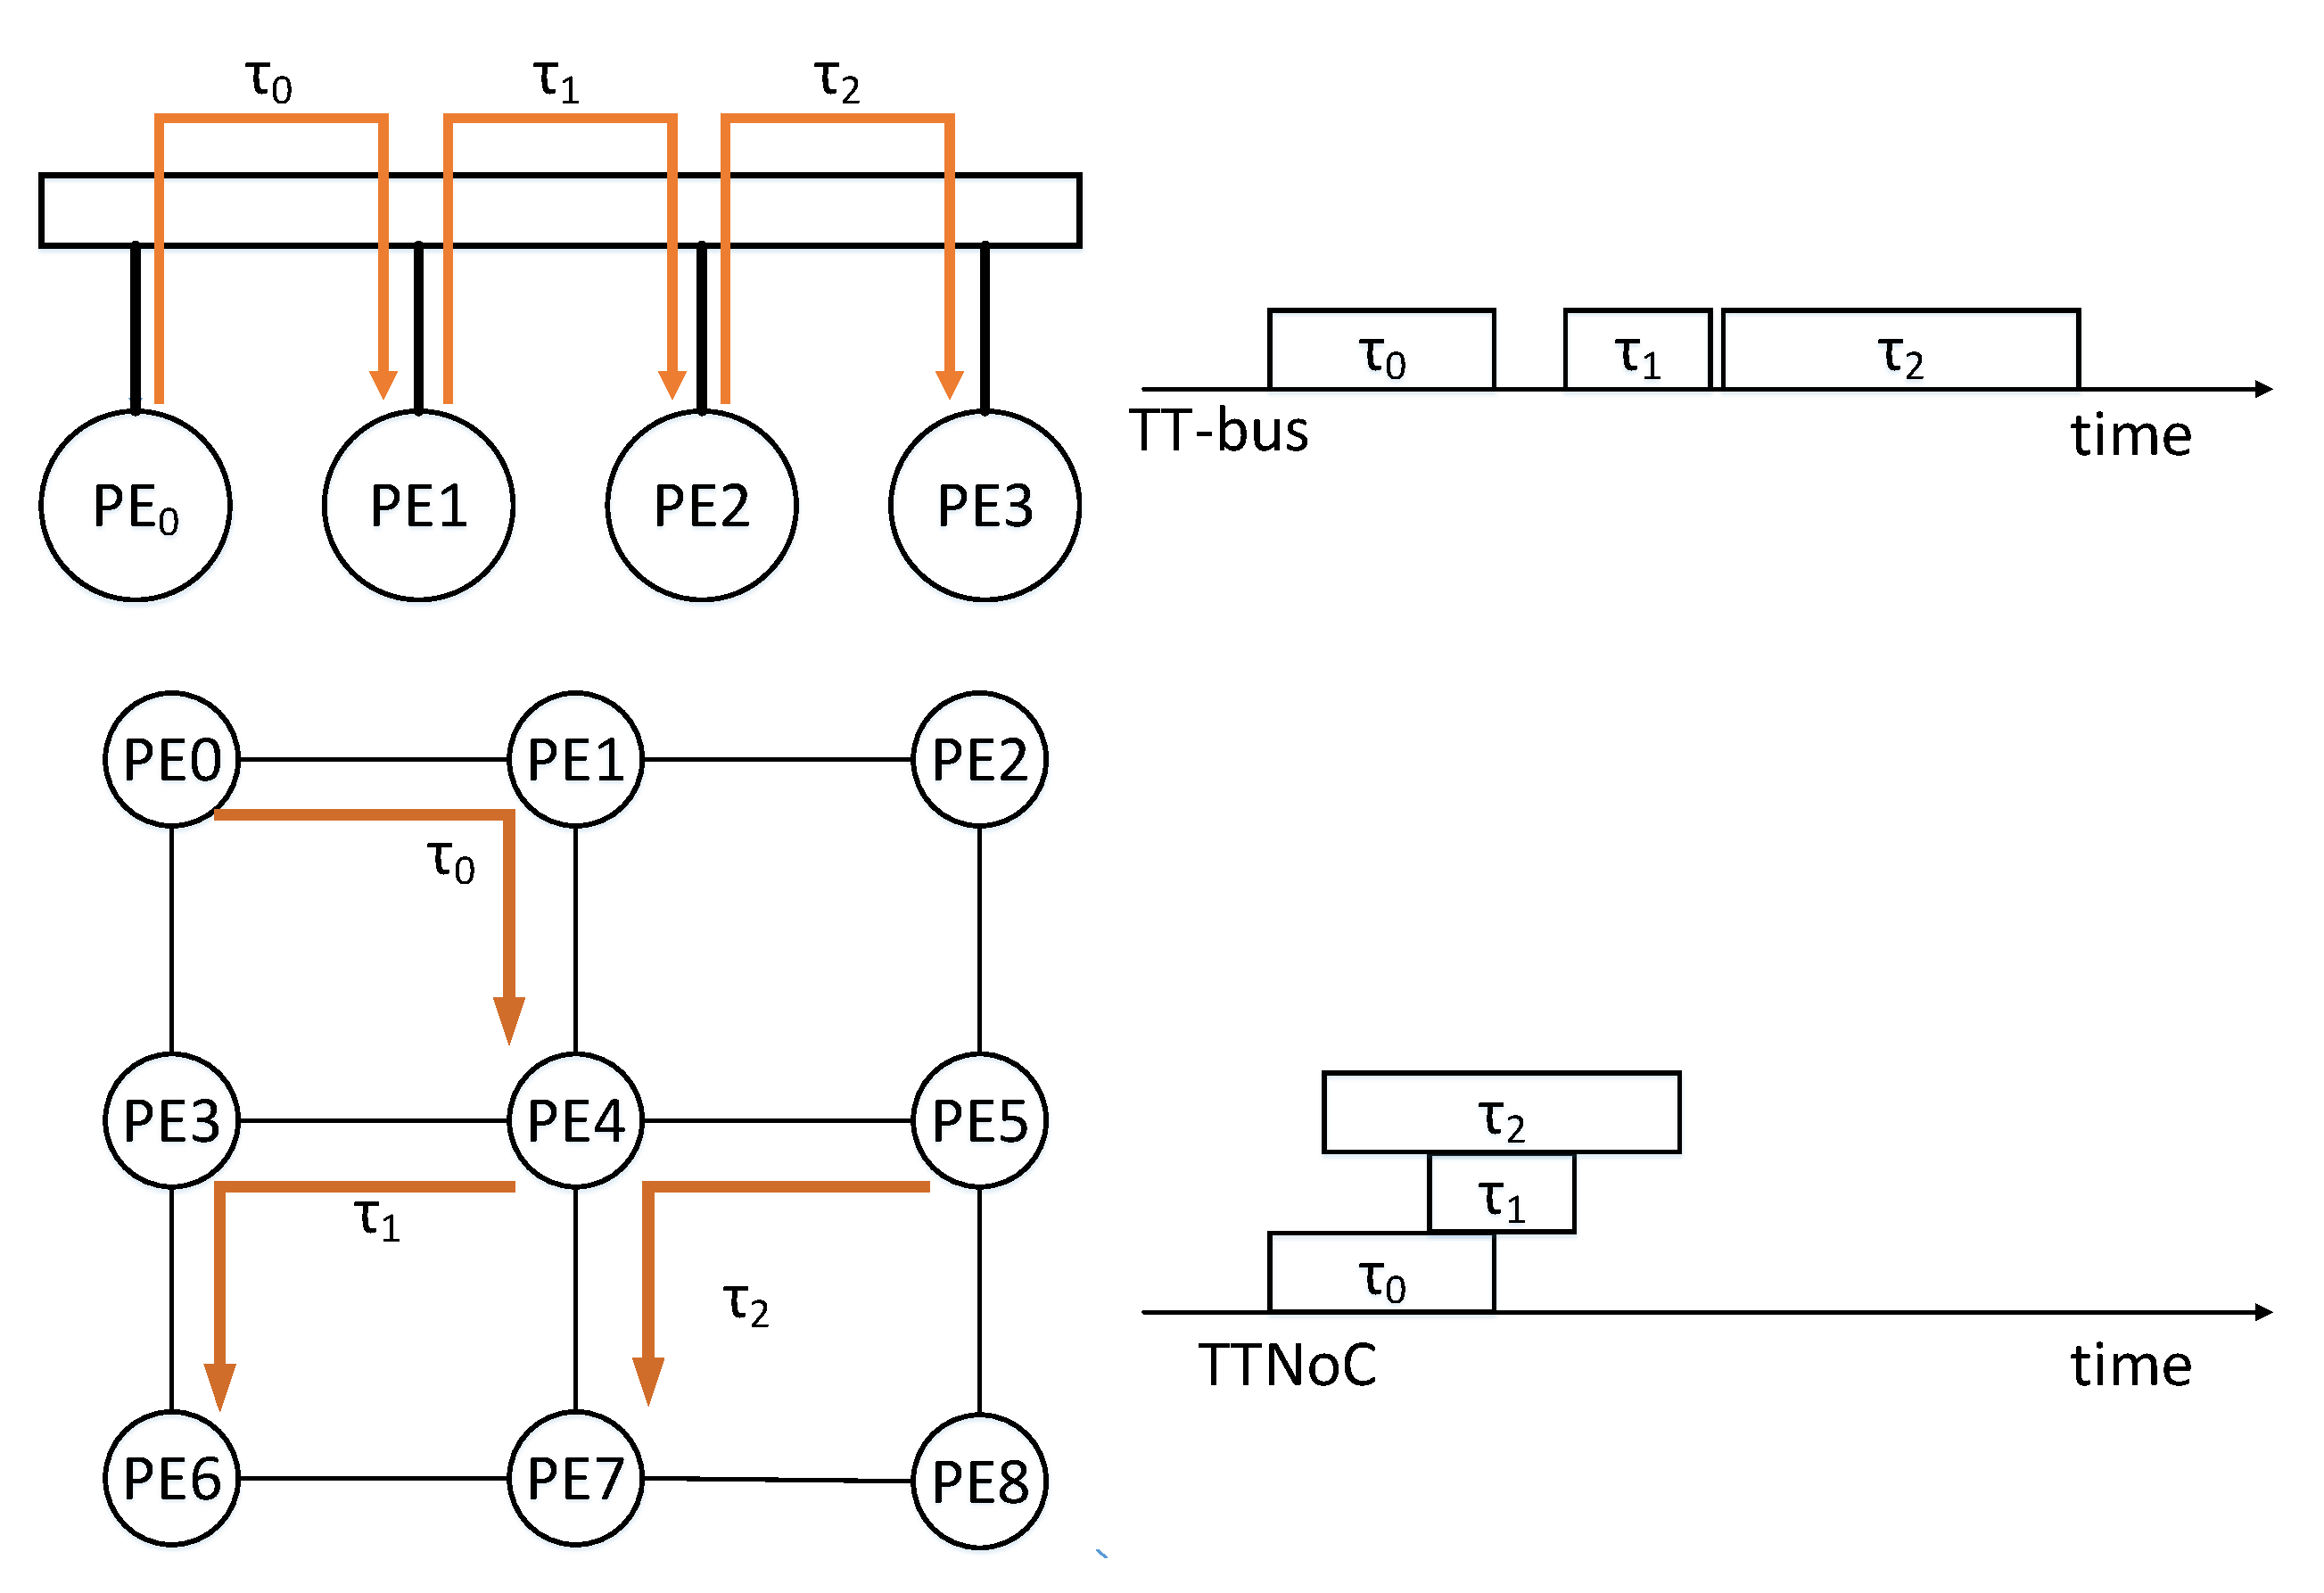
\includegraphics[width=3in]{picture/difference.pdf}
	\caption{Difference between bus- and network-based time-triggered architecture}
	\label{f:diff}
\end{figure}

The TTNoC is network-based, therefore the scheduling of TTNoC is to determine the duration of each message on the TTNoC and ensuring there is no contention with the communication. 
Static scheduling is adopted to synthesize the scheduling which resolves contention, avoiding dynamic arbitration of intercommunicate resources distribution. 
So that the communication on the TTNoC is predefined while satisfying the scheduling constrains.
However, synthesizing such a scheduling is rather complicated which is known as NP-complete~\cite{DBLP:conf/date/HuangBRBK12,DBLP:conf/rtss/Steiner10}.

The main contribution of this paper is presenting a static scheduling approach to resolve the TTNoC scheduling problem by the Memetic Algorithm (MA). MA is widely used as a synergy of evolutionary or any population-based approach with separate individual learning or local improvement procedures for solution search~\cite{DBLP:journals/tec/ChenOLT11}. 

The rest of this paper is organized as follows. We first review the related work in the TTNoC scheduling in Section~\ref{s:relate}. 
The system model is given in Section~\ref{s:model}, followed by the schedule constrains in Section~\ref{s:constraint}.
Next we presents the problem formulation and assumptions in Section~\ref{s:formulation}.
Then the memetic algorithm is described in Section~\ref{s:algorithm}.
The experiments as well as synthesis results are presented in Section~\ref{s:evalu}.
Finally, we conclude in Section~\ref{s:conclud}.

\section{Related Work	\label{s:relate}}

There are sufficient literatures about the scheduling of time-triggered network, which is similar to the scheduling of TTNoC. 
\cite{DBLP:conf/rtss/Steiner10} consider the scheduling problem for time-triggered multi-hop networks. A pure satisfiability modulo theories (SMT) formulation is presented followed by an incremental method to improve the scalability.
\cite{DBLP:journals/rts/CraciunasO16,DBLP:conf/rtns/CraciunasO14} formulate the schedule problem using first-order logical constraints and present alternative methods to find a solution based on SMT and mixed integer programming (MIP) solvers.
In \cite{DBLP:conf/etfa/PozoSRH15} the authors presents a decomposition approach based on SMT solver for extremely large time-triggered network.

The scheduling problem also appear in the various domain.
\cite{DBLP:conf/isorc/RoRM15} resolve the scheduling problem on the wireless network by SMT solver.
\cite{DBLP:conf/aspdac/ZhangG0C14} formulate the co-synthesis problem of task and communication schedules as a Mixed Integer Programming (MIP) model taking into account a number of Ethernet-specific timing parameters.
Holistic Scheduling in Time-Triggered In-Vehicle Networks was studied in~\cite{DBLP:journals/tii/HuLWLZ14}

The scheduling problem of TTNoC has been
studied firstly in \cite{DBLP:conf/date/HuangBRBK12} which is integrates SMT solver into classical heuristic algorithm. 
\cite{DBLP:conf/sies/ScholerKMO15} introduces an optimal scheduler based on a Boolean SAT solver for a TTNoC.
\cite{DBLP:conf/indin/MurshedOAK15} introduces a scheduling model based on Mixed Integer Linear Programming (MILP) combining both time-triggered and event-triggered messages on NoC.
In~\cite{DBLP:conf/sies/FreierC15},
 A heuristic algorithm for scheduling on the scalable communication structure like a NoC is presented. 


% An example of a floating figure using the graphicx package.
% Note that \label must occur AFTER (or within) \caption.
% For figures, \caption should occur after the \includegraphics.
% Note that IEEEtran v1.7 and later has special internal code that
% is designed to preserve the operation of \label within \caption
% even when the captionsoff option is in effect. However, because
% of issues like this, it may be the safest practice to put all your
% \label just after \caption rather than within \caption{}.
%
% Reminder: the "draftcls" or "draftclsnofoot", not "draft", class
% option should be used if it is desired that the figures are to be
% displayed while in draft mode.
%
%\begin{figure}[!t]
%\centering
%\includegraphics[width=2.5in]{myfigure}
% where an .eps filename suffix will be assumed under latex, 
% and a .pdf suffix will be assumed for pdflatex; or what has been declared
% via \DeclareGraphicsExtensions.
%\caption{Simulation results for the network.}
%\label{fig_sim}
%\end{figure}

% Note that the IEEE typically puts floats only at the top, even when this
% results in a large percentage of a column being occupied by floats.


% An example of a double column floating figure using two subfigures.
% (The subfig.sty package must be loaded for this to work.)
% The subfigure \label commands are set within each subfloat command,
% and the \label for the overall figure must come after \caption.
% \hfil is used as a separator to get equal spacing.
% Watch out that the combined width of all the subfigures on a 
% line do not exceed the text width or a line break will occur.
%
%\begin{figure*}[!t]
%\centering
%\subfloat[Case I]{\includegraphics[width=2.5in]{box}%
%\label{fig_first_case}}
%\hfil
%\subfloat[Case II]{\includegraphics[width=2.5in]{box}%
%\label{fig_second_case}}
%\caption{Simulation results for the network.}
%\label{fig_sim}
%\end{figure*}
%
% Note that often IEEE papers with subfigures do not employ subfigure
% captions (using the optional argument to \subfloat[]), but instead will
% reference/describe all of them (a), (b), etc., within the main caption.
% Be aware that for subfig.sty to generate the (a), (b), etc., subfigure
% labels, the optional argument to \subfloat must be present. If a
% subcaption is not desired, just leave its contents blank,
% e.g., \subfloat[].


% An example of a floating table. Note that, for IEEE style tables, the
% \caption command should come BEFORE the table and, given that table
% captions serve much like titles, are usually capitalized except for words
% such as a, an, and, as, at, but, by, for, in, nor, of, on, or, the, to
% and up, which are usually not capitalized unless they are the first or
% last word of the caption. Table text will default to \footnotesize as
% the IEEE normally uses this smaller font for tables.
% The \label must come after \caption as always.
%
%\begin{table}[!t]
%% increase table row spacing, adjust to taste
%\renewcommand{\arraystretch}{1.3}
% if using array.sty, it might be a good idea to tweak the value of
% \extrarowheight as needed to properly center the text within the cells
%\caption{An Example of a Table}
%\label{table_example}
%\centering
%% Some packages, such as MDW tools, offer better commands for making tables
%% than the plain LaTeX2e tabular which is used here.
%\begin{tabular}{|c||c|}
%\hline
%One & Two\\
%\hline
%Three & Four\\
%\hline
%\end{tabular}
%\end{table}


% Note that the IEEE does not put floats in the very first column
% - or typically anywhere on the first page for that matter. Also,
% in-text middle ("here") positioning is typically not used, but it
% is allowed and encouraged for Computer Society conferences (but
% not Computer Society journals). Most IEEE journals/conferences use
% top floats exclusively. 
% Note that, LaTeX2e, unlike IEEE journals/conferences, places
% footnotes above bottom floats. This can be corrected via the
% \fnbelowfloat command of the stfloats package.

\section{System Model}
\label{s:model}

In this section we presents the basis and model of TTNoC.
The system architecture we adopted is shown in~\cite{DBLP:conf/rtcsa/PaukovitsK08}. 

\subsection{Architecture Model}

TTNoC is a system with a set of real-time tasks/applications mapped on
a multi-core interconnection platform.  It composes of a set of
identical processing elements interconnected by physical links and the
switches on the TTNoC.  The switches are connected by bidirectional
physical links and each link connects a pair of switches.  The
topologies of a TTNoC can be either regular or irregular.

The architecture of a TTNoC is
modeled by a directed graph $\calG=(\calV,\calL)$. The set of vertexes
$\mathcal{V}=\{ v_{1},\dots,v_{m}\}$ represents the set of $m$
\emph{identical} communication nodes (the processing elements and
switches) while the edges $\mathcal{L}\subseteq \mathcal{V} \times
\mathcal{V}$ comprises the communication physical links
\emph{directly} connecting the nodes.  The physical links are
full-duplex, allowing thus communication in both
directions. Therefore, given $v_i,v_j\in\calV$, $\langle
v_i,v_j\rangle \in\calL$ implies $\langle v_j,v_i\rangle\in\calL$,
where $\langle v_i,v_j\rangle$ is a pair denoting a directed physical
link connecting two adjacent nodes, from a source node $v_i$ to a sink node $v_j$.

 
A TTNoC is composed of a set of identical process elements and
physical links.  Since the width of physical links as well as the
performance of switches and links is the same, the properties of each
hop can be regarded as system properties of TTNoC.  Thus a TTNoC
$\calG$ is equipped with a set of properties.  We use $\width$ to
denote the width of physical links in the TTNoC, $\SD$ for the
switching delay in the switches, $\HD$ for the link delay per hop
which means propagation cost between adjacent nodes, and $\MT$,
discussed in Section~\ref{ss:schmodel}, for the macrotick of network
representing the time-line granularity of the physical link.

%% A network link $(v_{a},v_{b})$, between the source node
%% $v_{a}$ and the sink node $v_{b}$, is defined by the tuple $\langle
%% (v_{a},v_{b}).w, (v_{a},v_{b}).sd,(v_{a},v_{b}).pd,(v_{a},v_{b}).mt,
%% (v_{a},v_{b}).h\rangle$, where $(v_{a},v_{b}).w$ is the width of
%% physical links, $(v_{a},v_{b}).sd$ is the switching delay in the
%% switches on network link, $(v_{a},v_{b}).pd$ is the link delay per hop
%% which means propagation cost between adjacent nodes,
%% $(v_{a},v_{b}).mt$ is the macrotick of network denotes the time-line
%% granularity of the physical link and $(v_{a},v_{b}).h$ is the number
%% of hops from $v_{a}$ to $v_{b}$ on the link $(v_{a},v_{b})$.

Given two nodes $v,v'\in\calV$, a \emph{route} from $v$ to $v'$,
denoted by $\route{r}{v}{v'}$, is defined as a sequence of the form
$\langle v_{k_0},v_{k_1}\rangle\langle
v_{k_1},v_{k_2}\rangle\ldots\langle v_{k_{i-1}},v_{k_i}\rangle\langle
v_{k_i},v_{k_{i+1}}\rangle\ldots \langle v_{k_{n-1}},v_{k_n}\rangle$
satisfying $v_{k_0}=v$, $v_{k_n}=v'$ and $(\forall i\in [1,n])\langle
v_{k_{i-1}},v_{k_i}\rangle \in\calL$. The length $n$ of the route is
written as $|\route{r}{v}{v'}|$. A route $\route{r}{v_i}{v_j}$
represents a \emph{possibly indirect} physical link from $v_i$ to
$v_j$ in the TTNoC, hence its length $|\route{r}{v_i}{v_j}|$ is the
number of hops along this link.

%% For a communication node $ \mathit{v}_{i}\in\mathcal{V} $, it offer
%% $\mathit{d}$ input links and $\mathit{d}$ output links, $\mathit{d}$
%% is the switch degree. Therefore a switch is able to connected with at
%% most $ \mathit{d} $ port in full-duplex connection. The adjoint
%% switches $v_{i}\in\mathcal{V}$ and $v_{j}\in\mathcal{V}$ which connect
%% with each other through physical link rather than the forwarding by
%% other switches, is defined by the sequence $ <v_{i},v_{j}>
%% $. Therefore the network link $(v_{a},v_{b})$ can be split in several
%% connection among the adjoint switches $v_{i}\in\mathcal{V}$, and we
%% have that $ (v_{a},v_{b})=\{ \langle v_{a},v_{1}> ,\dots,
%% <v_{i},v_{j}> ,\dots, <v_{n},v_{b}> \} $.  


\subsection{Message Model}
The communication of process elements on the TTNoC is based on
messages.  A message consists of header and data.  Header includes the
information for message forwarding on the TTNoC, e.g. the addresses of
source and destination.  A flit is the unit of a message that can be
transmitted over the TTNoC.  Only periodic messages are discussed in
this paper because it is the typical case in real-time embedded
systems.  But in practice, the fixed time slot can be preserved in
terms of the route and deadline periodically for sporadic messages.

We denote the set of $n$ time-triggered messages on the TTNoC by
$\Gamma = \{\tau_{1},\dots,\tau_{n}\}$. Each message $\tau_{i}$ is
modeled by the tuple $\langle \tau_{i}.H,\tau_{i}.S, \tau_{i}.T,
\tau_{i}.D\rangle$, 
where $\tau_{i}.H$ denotes the header of the message in flits,
$\tau_{i}.S$ denotes the size of the message in flits, 
$\tau_{i}.T$ and $\tau_{i}.D$ are the period and the relative deadline of the message, respectively.
 
\subsection{Scheduling Model}
\label{ss:schmodel}

When a communication happens on the TTNoC between two nodes, i.e. a
source node $v_i\in \calV$ sends a message $\tau_{k}$ to a sink node
$v_j\in \calV$ on the TTNoC, the message $\tau_k$ is transmitted on
some route $\route{r}{v_i}{v_j}$ and the communication nodes along the
route $\route{r}{v_i}{v_j}$ forward the message.

The TDMA scheme is deployed for the scheduling of communication.  And
the time granularity is \emph{macrotick} that the periods and the
phases of messages directly match to this time format.

Based on the architecture and message model, we can model the scheduling of communication as a set $\calS=\{s_1,\ldots,s_n\}$, in which each
$s_{i}$ denotes the communication scheduling of the message
$\tau_{i}\in\Gamma$. Each communication $s_{i}\in\calS$ is defined
using a tuple $\langle s_i.R, s_i.\phi, s_i.T, s_i.D, s_i.L\rangle$,
where $s_i.R$ is the route along which the message $\tau_i$ is
forwarded, 
$s_i.\phi$ is the offset of the communication, $s_i.T$ and
$s_i.D$ denote, 
respectively, 
the period and the relative deadline of the communication, and $s_i.L$ is the duration of the communication.

For the whole set $\calS$, the sets of the route, the period, the
relative deadline and the delay of each $s_i\in\calS$ are defined as
expected, denoted by $\calS.\calR$, $\calS.\Phi$, $\calS.\calT$,
$\calS.\calD$ and $\calS.\calL$, respectively.

%% Based on the architecture and message model, we can model the set of
%% message communication $\mathcal{M}=\{ s_{1},\dots,s_{i}\}$, where
%% $s_{i}\in\mathcal{M}$ denotes the communication scheduling of a
%% message $\tau_{i}\in\Gamma$. For each message $\tau_{i}\in\Gamma$ on
%% the link $(v_{a},v_{b}) $ where $v_{a},v_{b}\in\mathcal{V}$, we model
%% the communication $s_{i}\in\mathcal{M}$ as a tuple $\langle
%% s_{i}^{(v_{a},v_{b})}.\phi, s_{i}^{(v_{a},v_{b})}.\mathcal{T},
%% s_{i}^{(v_{a},v_{b})}.\mathcal{D},s_{i}^{(v_{a},v_{b})}.\mathcal{L}
%% \rangle$, where $ s_{i}^{(v_{a},v_{b})}.\phi$ is the offset of
%% communication, $ s_{i}^{(v_{a},v_{b})}.\mathcal{T} $ is the period of
%% communication, $s_{i}^{(v_{a},v_{b})}.\mathcal{D}$ is the relative
%% deadline of communication, $s_{i}^{(v_{a},v_{b})}.\mathcal{L}$ is the
%% duration of communication and $(v_{a},v_{b})$ in the tuple is the
%% network link for communication.

Because of the macrotick as the granularity of communication,
for each communication $s_{i}$,
we have the following formulas:
\begin{equation}
\label{e:eqn1}
  s_i.T = \lceil\frac{\tau_{i}.T}{\MT} \rceil
\end{equation}
\begin{equation}
\label{e:eqn2}
  s_i.D = \lceil\frac{\tau_{i}.D}{\MT}\rceil
\end{equation}
\begin{equation}
\label{e:eqn3}
  s_i.L = \lceil\frac{|s_i.R| \times (\SD+\HD) \times
    \lceil\frac{\tau_{i}.S + \tau_{i}.H}{\tau_{i}.H  }\rceil}{\MT}\rceil
%\lceil\frac{\tau_{i}.s\times (v_{a},v_{b}).sc+(v_{a},v_{b}).delay}{ (v_{a},v_{b}).mt}\rceil 
\end{equation}
%% where $(v_{a},v_{b}).d = (v_{a},v_{b}).sd+(v_{a},v_{b}).pd $ denotes
%% the delay of propagating and switching delay per hop.
where $\MT$ denotes the value of macrotick, and $\SD+\HD$ is the delay
per hop in the forwarding.
%% that $\SD$ is the delay on the physical link and $\HD$is the switching delay.

The formula is based on~\cite{DBLP:books/daglib/0087651} with the
modification of adopting macrotick as the unit.  Given an
$s_{i}\in\calS$ and its route $s_i.R$, $s_i.T$, $s_i.D$ and $s_i.L$
can be derived by formulas~\ref{e:eqn1}, \ref{e:eqn2}
and~\ref{e:eqn3}.  Formulas~\ref{e:eqn1} and~\ref{e:eqn2} denote,
respectively, the period and the deadline of the communication $s_i$
in macrotick.  Formula~\ref{e:eqn3} computes the time cost in
macrotick, from the first flit sent by the source node to the last
flit received by the sink node, according to the store-and-forward
(SAF) switching scheme~\cite{DBLP:books/daglib/0087651}.  Moreover,
other scheme of switching on the NoC can be also deployed in the TTNoC
according to the requirements. In this case, the delay formula
\ref{e:eqn3} should be changed according to the given switching
scheme.

As a result, to synthesize the set of communication $\calS$ is to
calculate the offset $s_i.\phi$ for each communication
$s_i\in\calS$. Therefore, the key to scheduling of TTNoC is to derive
$\calS.\Phi = \{s_i.\phi\mid s_i\in\calS\}$ based on the given
architecture model $\calG$ and the messages model $\Gamma$ with
\emph{scheduling constraints}.


\section{Scheduling Constraints\label{s:constraint}}

The scheduling constraints for general time-triggered multi-hop
network are presented in~\cite{DBLP:conf/rtss/Steiner10}.  The
scheduling constraints on TTNoC are similar with those on general
time-triggered network, while some differences exist in terms of our
model.

Scheduling of communication $\calS$ should resolve the constraints on
the TTNoC. \jx{This statement is unclear:}  The synthesized scheduling must satisfy the separation
among the set of communication in time domain or space domain, which
mainly include offset constraints and link constraints.

In our TTNoC, scheme of bufferless NoCs is adopted that no buffering
of messages takes place.  It leads to significantly less area and
power consumption for TTNoC~\cite{DBLP:journals/tpds/ShpinerKLCK15}.
The route of each message is located on its header.  The switches
simply forward the message according to the address of next-hop
switch, without concerning the communication schedule. Therefore,
unlike the general time-triggered network, the switch memory
constraints are not concerned. \jx{Check this sentence:} Moreover for
the simplicity of evaluation, the constraints of simultaneous relay,
application-level, protocol-based and domain-specific are neither
concerned.

\subsection{Message Offset Constrains}

For a scheduling of message $s_{i}\in\calS$ , the offset $s_i.\phi$  must be positive values and should guarantee that the message transmission is completed before the deadline of the communication. Therefore we have that
\begin{equation}
	(s_i.\phi
	\geq 0)
	\cap
	(s_i.\phi + s_i.L
	\leq
	s_i.D)
\end{equation}

\subsection{Link Contention Constrains}

For each communication, the message occupies the link in terms of routing strategy without contention, 
until all the message is received by sink node.
The scheduling $\calS$ should guarantee that no two messages that are both transmitted on the identical link time at any time. 
The synthesized scheduling must guarantee that the links on TTNoC is contention-free.

Therefore for any two of the scheduling of message 
$s_i,s_j\in\calS,s_i\neq s_j$,
%$s_{i},s_{j}\in\mathcal{M}, s_{i}\neq s_{j}$, 
we define 
%$ overlap(s_{i},s_{j}) $,
$ overlap(s_i,s_j)$
 denotes whether there is common routing link between $s_i$ and $s_j$ or not. 
$ overlap(s_i,s_j)$ equals 1 if two communications sharing routing link for at least one hop. 
Therefore we have that
\begin{equation}
\label{e:overlap}
overlap(s_i,s_j)= 
	\begin{cases}
	0 \quad s_i.R \cap s_j.R = \emptyset\\
	1 \quad s_i.R \cap s_j.R \neq \emptyset
\end{cases}
\end{equation}

The duration of scheduling $s_i$ for message $\tau_i$ in its $\mathit{k}$th period is defined by $s_i(k)$, which equals
\begin{equation}
\label{e:duration}
	s_i(k)
	=
	[
	k\times s_i.T+s_i.\phi
	,
	k\times s_i.T+s_i.\phi+s_i.L
	%{s_{i}^{(v_{a},v_{b})}}.\mathcal{T}+{s_{i}^{(v_{a},v_{b})}}.\phi+{s_{i}^{(v_{a},v_{b})}}.\mathcal{L}			
	]
\end{equation}

Therefore for any 
$	s_i,s_j \in \calS, s_i \neq s_j	$,
%$ {s_{i}^{(v_{a},v_{b})}}\in\mathcal{M}, {s_{j}^{(v_{c},v_{d})}}\in\mathcal{M}$,
we have that
\begin{equation}
	s_i.R \cap s_j.R \neq \emptyset
	\Longrightarrow
	s_i(p) \cap s_j(q) = \emptyset
\end{equation}
%\begin{equation}
%	(v_{a},v_{b})
%	\cap
%	(c_{c},v_{d})
%	\neq
%	\emptyset
%	\Longrightarrow
%	{s_{i}^{(v_{a},v_{b})}}(p)
%	\cap
%	{s_{j}^{(v_{c},v_{d})}}(q)
%	=
%	\emptyset	
%\end{equation}
where $p,q\geq 0$, $p,q\in\mathcal{Z}$.

\section{PROBLEM FORMULATION\label{s:formulation}}
The problem we are addressing in this paper can be formulated as follow. Given:
\begin{itemize}
	\item The architecture of TTNoC $\calG=(\calV,\calL)$ consists of the set of communicating nodes $\mathcal{V}=\{\mathit{v}_{1},\dots,\mathit{v}_{m}\}$ and interconnection links $\mathcal{L}=\{ \langle v_i,v_j  \rangle \mid  v_i,v_j \in \calV\}$.
	\item The mapping of message to communication node
		$\{<\tau_{i},v_{j}>\mid \tau_{i}\in\Gamma,v_{j}\in\mathcal{V}$\}. 
		Each message $\tau_{i}\in\Gamma$ is allocated to a specific process element(communication node) $v_{i}\in\mathcal{V}$, 
		thus the source node $v_{a}$ and sink node $v_{b}$ for each $\tau \in\Gamma$ are determined.
		It should be noted that the scheduling of mapping can be synthesized by genetic algorithm~\cite{DBLP:conf/recosoc/MesidisI11}.
		In our experiment the mapping is predefined.
	\item The set of tt-messages $ \Gamma = \{\tau_{1},\dots,\tau_{n} \}$ with 
	$\langle \tau_{i}.H,\tau_{i}.S, \tau_{i}.T,	\tau_{i}.D\rangle$ for each $\tau \in \Gamma$.
	\item The route $s_i.R$ for each scheduling $s_i \in \calS$ of message $\tau \in \Gamma$.
\end{itemize}
%(1) the architecture of  network $\mathcal{G}=(\mathcal{V},\mathcal{L})$ consists of the set of communicating nodes $\mathcal{V}=\{\mathit{v}_{1},\dots,\mathit{v}_{m}\}$ and interconnection links $\mathcal{L}=\{ (v_{a},v_{b}) \mid  v_{a},v_{b}\in \mathcal{V}\}$.
%(2) the mapping of message to communication node $\{<\tau_{i},v_{j}>\mid \tau_{i}\in\Gamma,v_{j}\in\mathcal{V}$\}. 
%(3) the routing strategy.
%(4) the set of tt-messages $ \Gamma = \{\tau_{1},\dots,\tau_{n} \}$ with  $\langle \tau_{i}.s, \tau_{i}.t, \tau_{i}.d\rangle$ for $\tau_{i}\in \Gamma$.
We aim to find the offset $\calS.\Phi$ for messages $\Gamma$ on TTNoC $\calG=(\calV,\calL)$ which satisfy the scheduling constrains. 

We introduce the memetic algorithm to synthesize the set of offset $\calS.\Phi$ such that satisfies the scheduling constrains. 
If it is impossible to synthesize a set of scheduled communication, 
then we try to minimize the amount of infeasible messages which violate the scheduling constrains.
% $\mathcal{M} = \{s_{1},\dots,s_{i}\}$ for each $\tau_{i}\in \Gamma $ to satisfy the set of given scheduling constrains. 

%Deriving the set of communication scheduling $\mathcal{M}$ means determine $\langle s_{i}^{(v_{a},v_{b})}.\phi, s_{i}^{(v_{a},v_{b})}.\mathcal{T}, s_{i}^{(v_{a},v_{b})}.\mathcal{D},s_{i}^{(v_{a},v_{b})}.\mathcal{L} \rangle$ for each $s_{i}\in \mathcal{M}$. The $s_{i}^{(v_{a},v_{b})}.\mathcal{T}$,$s_{i}^{(v_{a},v_{b})}.\mathcal{D}$ and $s_{i}^{(v_{a},v_{b})}.\mathcal{L}$ can be derived easily through formula (1),(2) and (3), respectively. Nevertheless, our goal is to find the set of offset $\mathcal{M}.\Phi$ such that satisfies the offset and link constrains. If it is impossible to synthesize a set of scheduled communication, then we try to minimize the amount of infeasible messages which violate the scheduling constrains.



\section{MEMETIC ALGORITHM\label{s:algorithm}}

Memetic algorithm(MA) is a population-based hybrid genetic algorithm(GA) coupled with an individual learning procedure capable of performing local refinements\cite{DBLP:journals/cim/OngLC10}. 

Our memetic algorithm consists of two parts. We deploy the genetic algorithm as global searching for the set of communication to be scheduled. And choosing the subset of infeasible communications as the element to local search.

The MA requires genetic representation, fitness function as well as evolution strategy, i.e. crossover, mutation and local search. We firstly give an example of communication scheduling to explain the genetic representation. Next the pseudocode is shown. And then the detail will be discussed.
\subsection{An Example of Scheduling on TTNoC}

To show our memetic algorithm,
 we firstly give an example of scheduling $\calS$ of messages $\Gamma$ on a $3\times 3$ mesh NoC,
 shown in Fig~\ref{f:comm_on_TTNoC}. 
There are a set of message to be scheduled on the TTNoC,
 we derive the scheduling model employing the architecture and message model,
 shown in TABLE~\ref{t:comm_info}.
%$\mathcal{\calS = \{s_{0},s_{1},s_{2},s_{3},s_{4}\}$ to be scheduled. 
Each scheduling $s_i\in\calS$ own its period, duration as well as link in terms of the given route.
It is noted that the period must be a positive power of two in terms of macrotick according to the timing specification of TTNoC~\cite{DBLP:conf/date/HuangBRBK12}.

We assume that the relative deadline is equal to period for each message for simplicity.
The set of possible offset is denoted as $s_i.\Phi$ for $s_i\in\calS$.
$s_i.\Phi$ is derived by $ 0 \leq s_{i}.\phi \leq s_{i}.T - s_{i}.L $ according to the message offset constrains.
The $s_i.\phi$ is generated among the $s_i.\Phi$.
The set of possible offset $s_i.\Phi$ for the messages on Fig~\ref{f:comm_on_TTNoC} is also shown in TABLE~\ref{t:comm_info}.
\begin{figure}[!t]
	\centering
	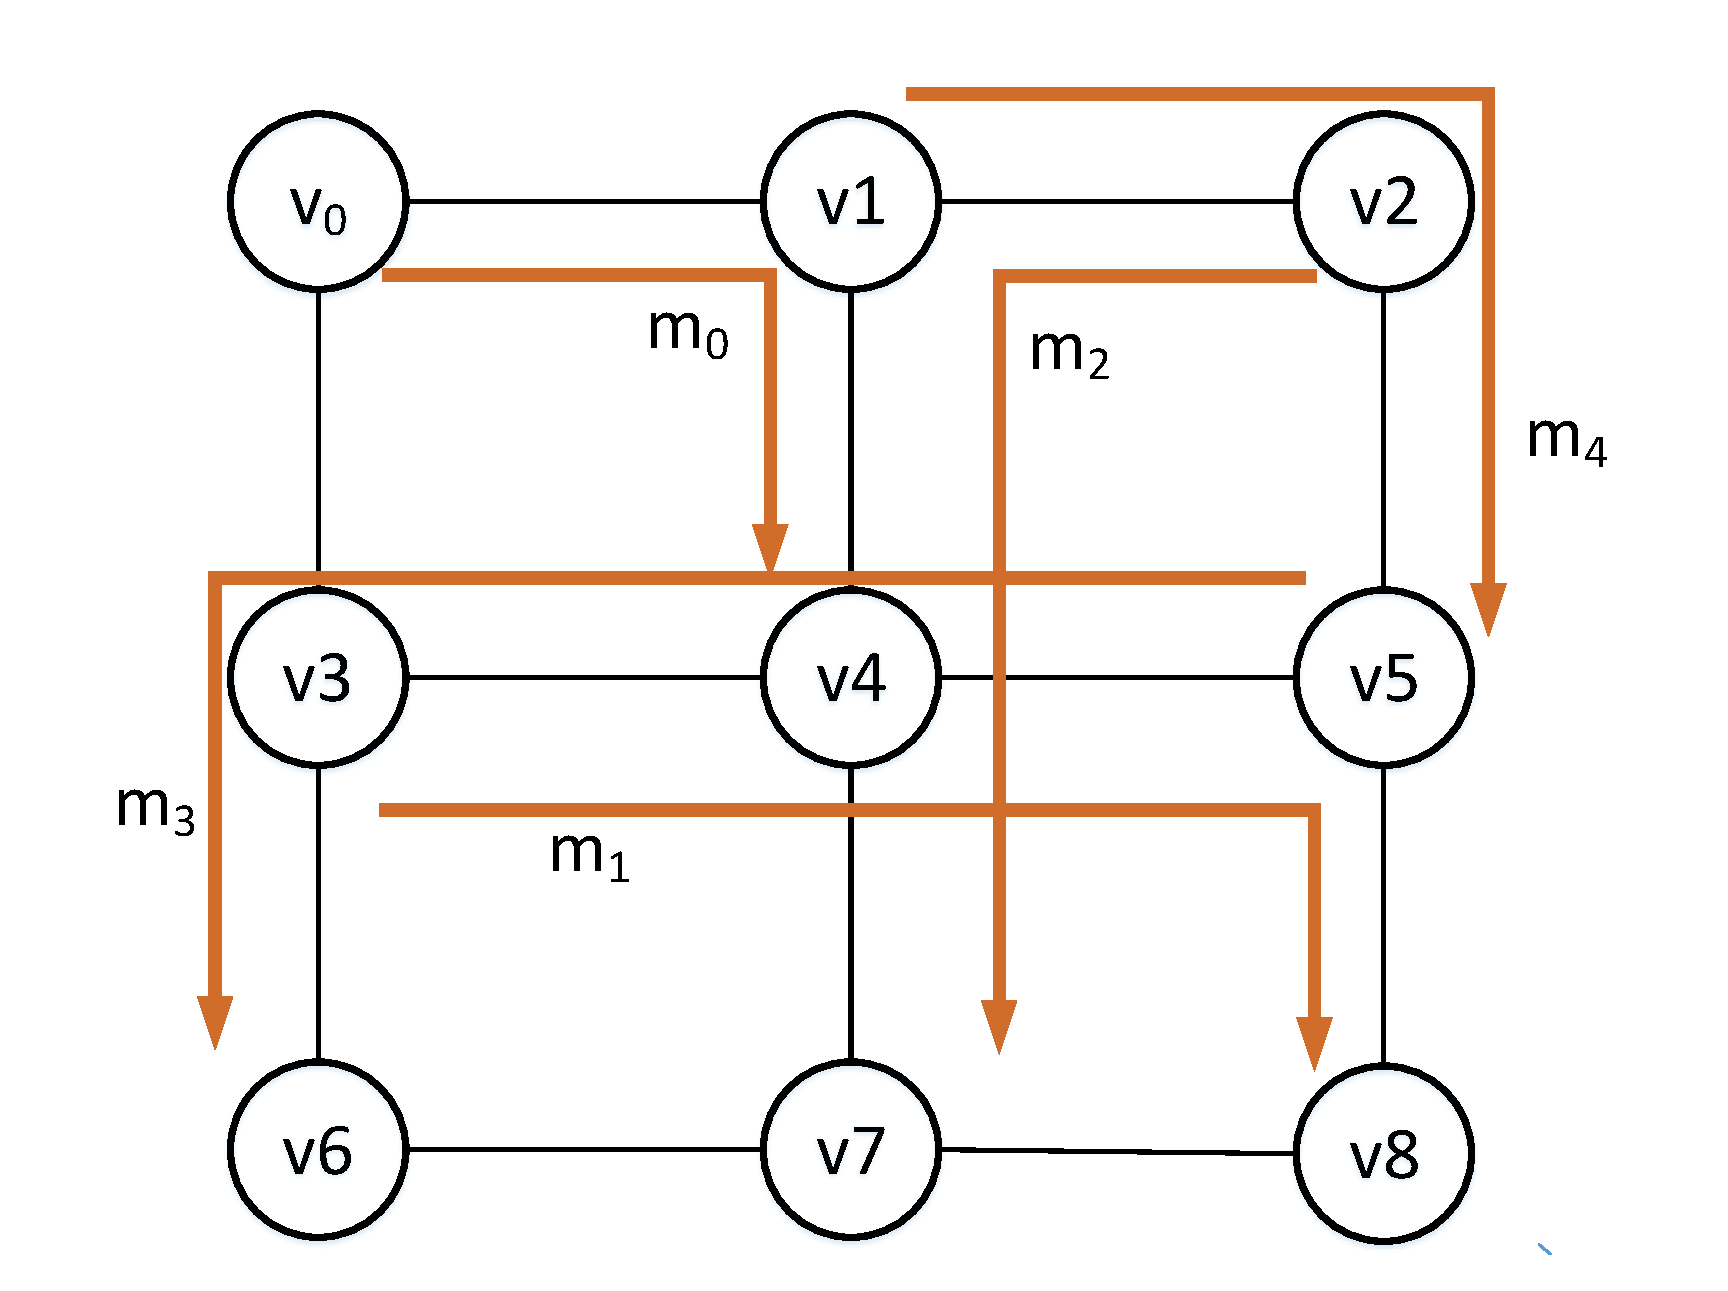
\includegraphics[width=2.5in]{picture/scheduling_example.pdf}
	\caption{An example of communication on the TTNoC}
	\label{f:comm_on_TTNoC}
\end{figure}
\begin{table}[!t]
	\renewcommand{\arraystretch}{1.3}
	%if using array.sty, it might be a good idea to tweak the value of
	% \extrarowheight as needed to properly center the text within the cells
	\caption{An Example of scheduling of messages on the TTNoC}
	\label{t:comm_info}
	\centering
	% Some packages, such as MDW tools, offer better commands for making tables
	% than the plain LaTeX2e tabular which is used here.
	\begin{tabular}{|c||c||c||c||c|}
		\hline
			\textbf{Scheduling } & 
			\textbf{Route } & 
			\textbf{Period} & 
			\textbf{Delay } & 
			\textbf{Possible Offset}\\
		\hline
		$s_{0}$ & $ r^{(0,4)} $ & 2 & 1 & $\{0,1\}$\\
		\hline
		$s_{1}$ & $ r^{(3,8)} $ & 4 & 1 & $\{0,1,2,3\}$\\
		\hline
		$s_{2}$ & $ r^{(2,7) }$ & 4 & 1 & $\{0,1,2,3\}$\\
		\hline		
		$s_{3}$ & $ r^{(5,6) }$ & 8 & 2 & $\{0,1,2,3,4,5,6\}$\\
		\hline
		$s_{4}$ & $ r^{(1,5) }$ & 8 & 1 & $\{0,1,2,3,4,5,6,7\}$\\
		\hline		
	\end{tabular}
\end{table}
\subsection{Genetic Representation}

The genetic algorithm employs global search consists of gene, chromosome,
 individual and population. 
The population consists of a set of individual and each contains a chromosome which represents a solution to the given question. 
A chromosome composes of several gene,
 which is the unit of chromosome.
We define them on the scheduling on the TTNoC.

In our memetic algorithm,
 we adopt hyperperiod  $H(\calS) = LCM\{\calS.\calT\}$
 as the chromosome definition.
Hyperperiod is the least common multiple of the offset among scheduling for messages. 
And the macrotick is defined as the unit of hyperperiod which is called gene.
The length of chromosome equals the value of $H(\calS)$,
 e.g. the hyperperiod is 8 for the scheduling set on TABLE~\ref{t:comm_info}. 

The location of a gene on the chromosome denotes the offset $ s_i.\phi $ of a message $\tau_i\in\Gamma$.
The offset of scheduling is distributed on a gene.
Therefore each chromosome on different individual represents a possible allocation of the offset set $\calS.\Phi$.
It should be noted that a single gene may consists multiple offset of messages,
 since several communication is able to offset at same time based on the TTNoC architecture if the TTNoC is out of contention.

A set of individual with respective chromosome composes the population.
The size of population equals the number of individual.
An example of population with two individual,
 based on TABLE~\ref{t:comm_info},
  is shown in TABLE~\ref{t:pop}.
And the example of chromosome and gene is also depicted.
%\begin{figure}[!t]
%	\centering
%	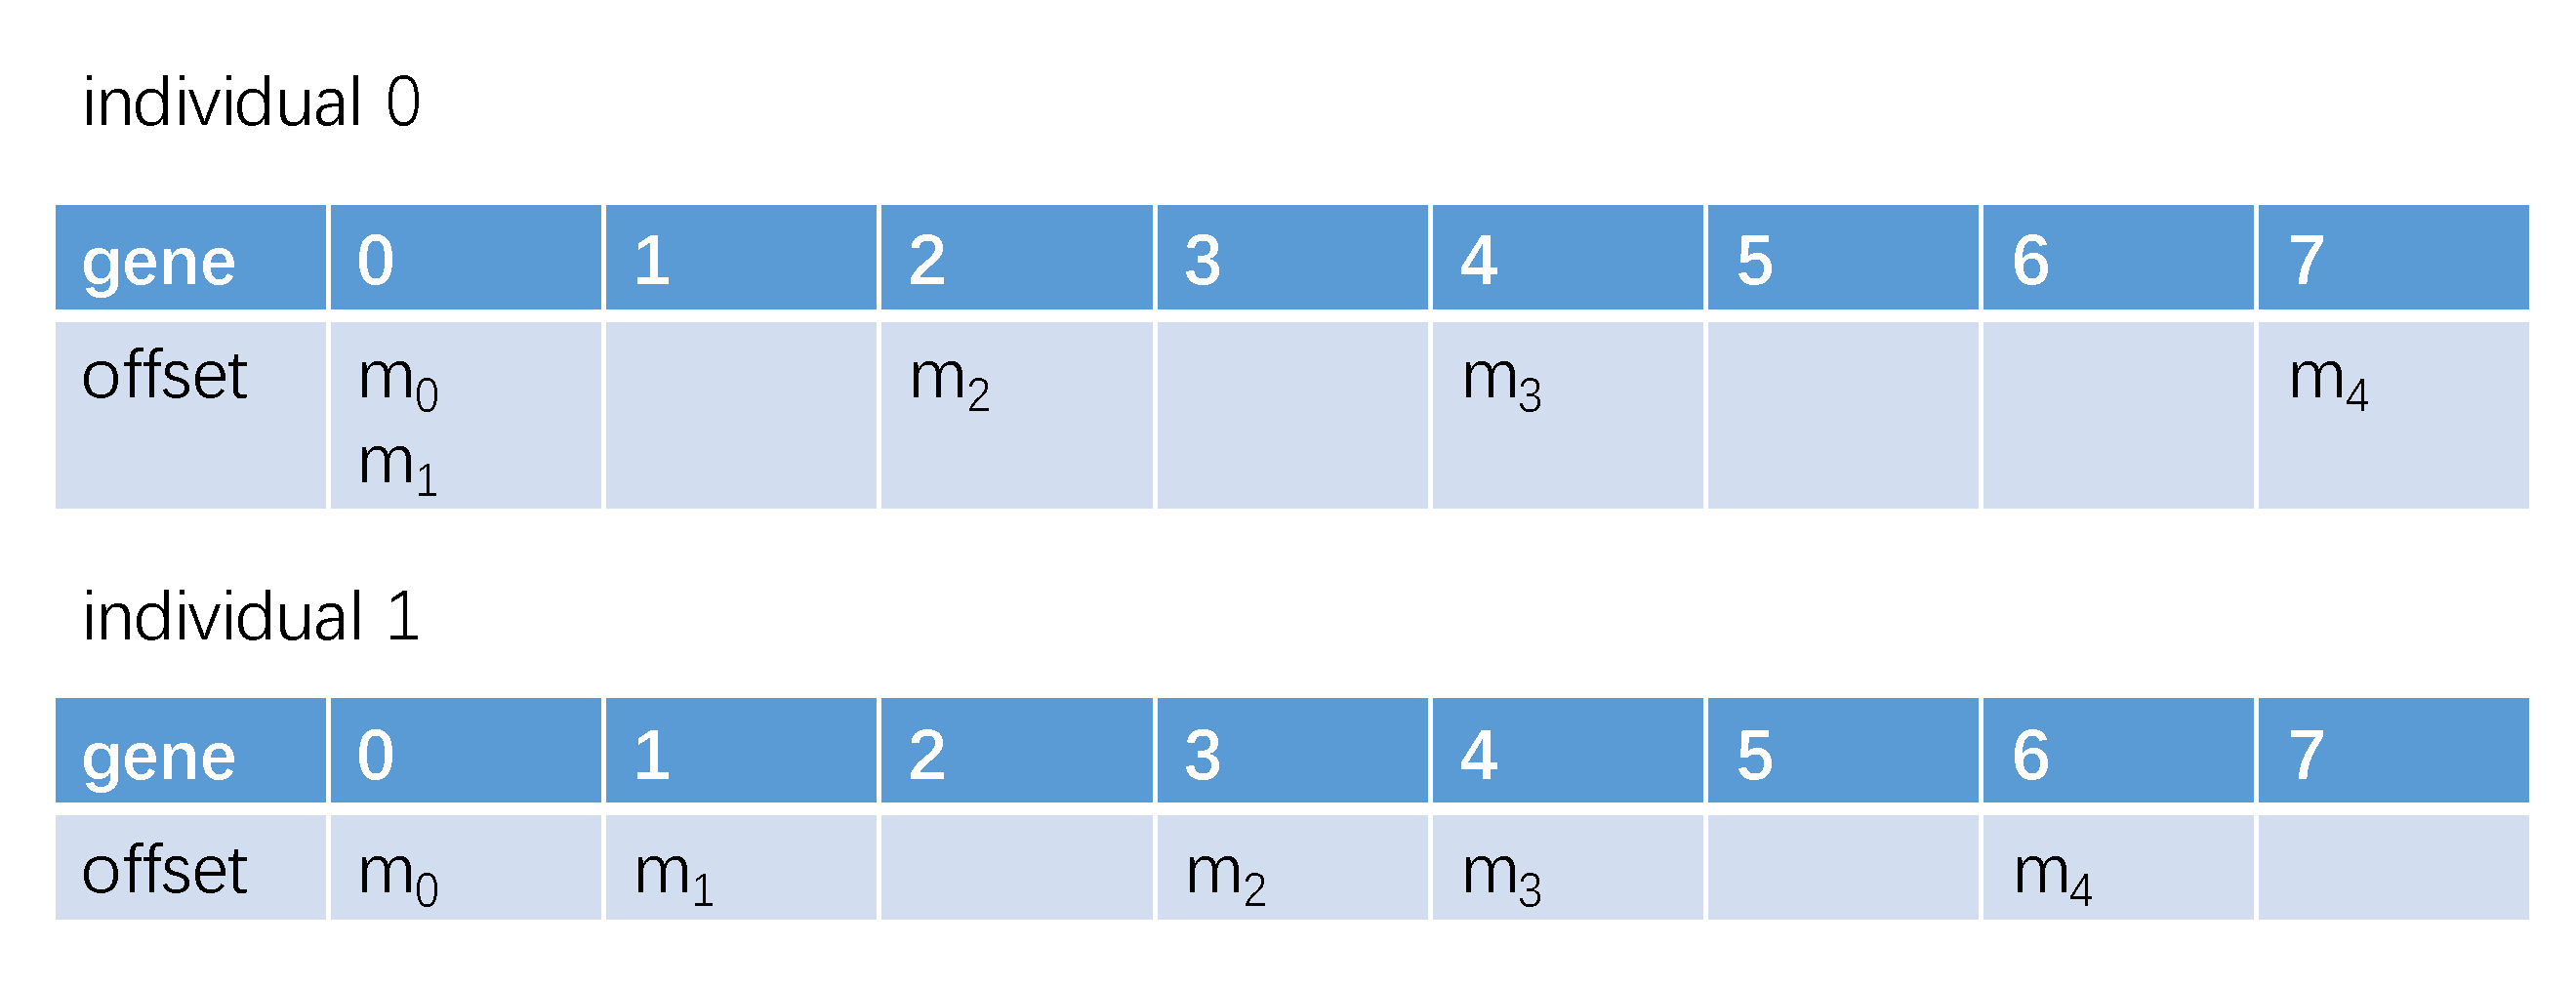
\includegraphics[width=3 in]{picture/2individual}
%	\caption{An example of population with 2 individual}
%	\label{t:pop}
%\end{figure}
\begin{table}[!t]
	\renewcommand{\arraystretch}{1.3}
	%if using array.sty, it might be a good idea to tweak the value of
	% \extrarowheight as needed to properly center the text within the cells
	\caption{An Example of population with 2 individual}
	\label{t:pop}
	\centering
	% Some packages, such as MDW tools, offer better commands for making tables
	% than the plain LaTeX2e tabular which is used here.
	\begin{tabular}{|c||c||c||c||c||c||c||c||c|}
	\hline
		\textbf{Gene}& 
		\textbf{0} & 
		\textbf{1} & 
		\textbf{2} & 
		\textbf{3} &
		\textbf{4} & 
		\textbf{5} & 
		\textbf{6} & 
		\textbf{7} \\		
	\hline
		$indi0$	&$m_0,m_1$&	&$m_2$&	&$m_3$& & &$m_4$\\		
	\hline		
		$indi1$	&$m_0$&$m_1$&	&$m_2$&$m_3$& &$m_4$&	\\		
	\hline
	\end{tabular}
\end{table}
\subsection{Algorithm Description}

According to the genetic representation, we formal give the algorithm process. The pseudocode is given as follow.

The memetic algorithm begins with an initial population $Pop$. The size of population $scale$ as well as the maximum iterations $maxIteration$ is predefined.
The initial population is synthesized randomly.
For a scheduling $s_{i}\in\calS$,
 the offset $s_i.\phi$ in the initial individual is located randomly among the possible offset $s_i.\Phi$.
Therefore the initial population satisfies the offset constrains.
The algorithm is iterative executed until a feasible scheduling is found or reaching the given maximum iteration.

When the memetic algorithm get started, firstly the initial population is marked by the fitness function.
The score evaluating chromosome of the individual is assigned to individual.
The less the number of score, the better the individual.
Therefore the individual with score equals zero represents a feasible scheduling is synthesized.
The detail of fitness function is discussed in subsection \ref{s:fit}.

Next, the operation of genetic algorithm,
 i.e. crossover and mutation,
  is deployed as global search.
And after that the local search is adopted to the population if there are no feasible scheduling(individual with score of 0).
The detail of search strategy deployed in global as well as local search, is discussed in \ref{s:glo} and \ref{s:loc}, respectively.

After the global and local search,
 each individual in the population is evaluated by fitness function again.
And the new population for the next iteration is generated by selection according to the score of each individual.
The individual with less score own more possibility to reserve for the next population.
The selection function ensure the size of population is equal to the value of $scale$ in each iteration.

\begin{algorithm}[tb]
	\caption{Memetic Algorithm}
	\renewcommand{\algorithmicrequire}{\textbf{Input:}}
	\renewcommand{\algorithmicensure}{\textbf{Output:}}
	\begin{algorithmic}[1]
		\REQUIRE~~\\
		the size of population $scale$\\
		maximum iterations $maxIteration$\\
		\ENSURE~~\\
		Best scheduling $\calS$\\
		\FOR {$i = 0$ to $maxIteration-1$}
			\IF{$i=0$}
			\STATE /*mark the initial population*/
				\STATE generate the	initial population $initialPop$\\
				\STATE mark$(initialPop)$
				\STATE $\mathcal{S}$ = individual with least score \textbf{in} $initialPop$
				\STATE $Pop = initialPop$
			\ELSE
			\STATE /*global search*/
				\STATE crossover($Pop$)
				\STATE mutation($Pop$)
				\STATE mark$(Pop)$
			\ENDIF
			\STATE /*choose the individual best so far after global search*/
			\FORALL {individual $indi$ \textbf{in} $Pop$}		
				\IF{$indi.score<\mathcal{S}.score$}
					\STATE $\mathcal{S}=indi$
				\ENDIF
				\IF{$\mathcal{S}.score==0$}
					\STATE break
				\ENDIF
			\ENDFOR	
			\STATE localSearch($Pop$)
			\STATE mark$(Pop)$
			\STATE /*choose the individual best so far after local search*/
			\FORALL {individual $indi$ \textbf{in} $Pop$}		
				\IF{$indi.score<\mathcal{S}.score$}
					\STATE $\mathcal{S}=indi$
				\ENDIF
				\IF{$\mathcal{S}.score==0$}
					\STATE break
				\ENDIF
			\ENDFOR			
			\STATE select($Pop$, $scale$)
		\ENDFOR
		\RETURN {$\mathcal{S}$}
	\end{algorithmic}
\end{algorithm}	

\subsection{Fitness function \label{s:fit}}

To adopt the fitness function to evaluate individuals,
 we firstly transform chromosome to represent the duration of communication in a hyperperiod.
Next we derive the link contention constrains among the scheduling according to the routing strategy,
 as the basis of our fitness function.
Then the score of each individual is able to employed by fitness function.

For each scheduling $s_i \in \calS$ for the messages on the TTNoC,
 The delay of scheduling $s_i$ in $k$th period $s_i(k)$, is defined by formula~\ref{e:duration}.
And we have that
\begin{equation}
	s_i.H = \{ s_i(k) \mid k \in [ 0, H(\calS)/s_i.T - 1 ] \}
%s_{i}.\mathcal{H} = \{ {s_{i}^{(v_{a},v_{b})}}(k) \mid k \in [0, \mathcal{M.H} / s_{i}.\mathcal{T} - 1] \}
\end{equation}
where $s_i.H$ denotes the duration of a scheduling in hyperperiod.
We define 
 $ \calS.\calH = \{ s_i.H \mid s_i \in \calS \}$
%$\mathcal{M.H}=\{ s_{i}.\mathcal{H} \mid s_{i}\in \mathcal{M} \}$,
 denotes the set of duration for each message scheduling in hyperperiod. 
Therefore,
 the complete duration in hyperperiod for each scheduling $ \calS.\calH $ is determined.
TABLE~\ref{t:duration} is an example of the complete duration in a hyperperiod,
 based on two individuals in TABLE~\ref{t:pop}.
The scheduling model of messages is shown in TABLE~\ref{t:comm_info}.

%\begin{figure}[!t]
%	\centering
%	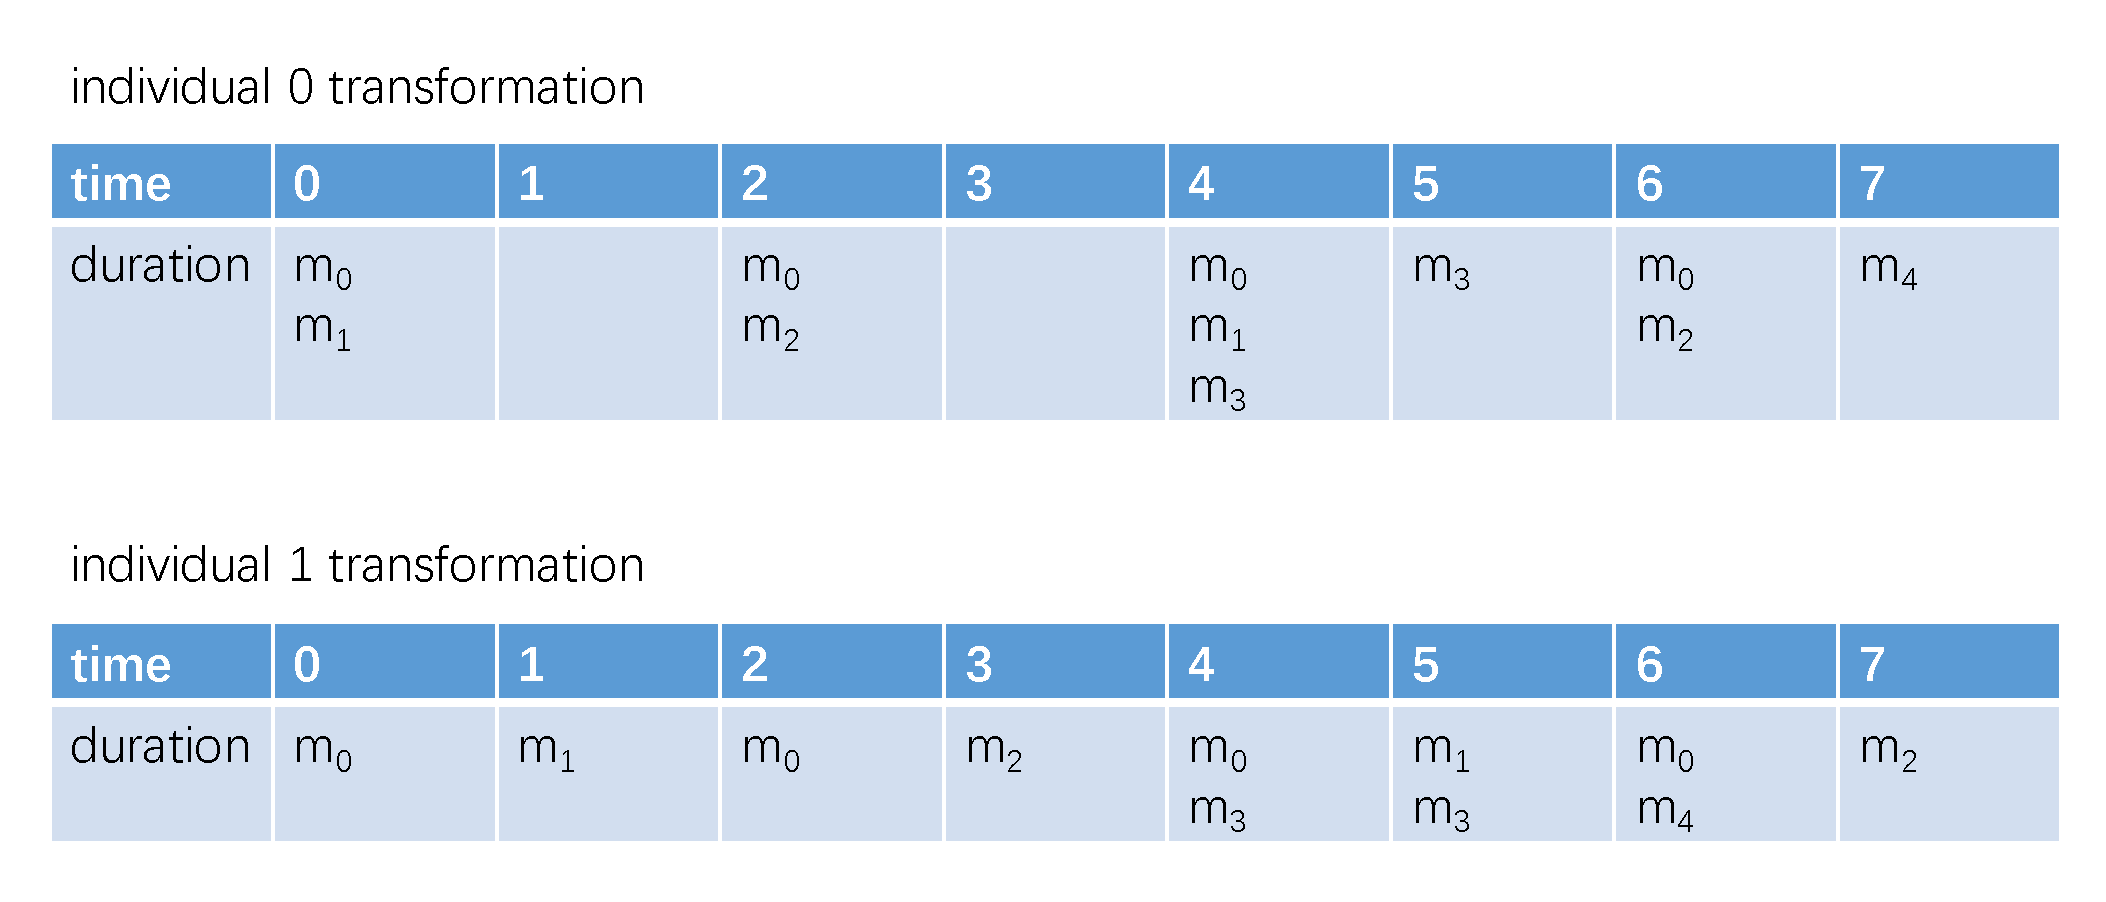
\includegraphics[width=3in]{picture/individual_transformation.pdf}
%	\caption{The duration of the messages in the hyperperiod}
%	\label{f:duration}
%\end{figure}
\begin{table}[!t]
	\renewcommand{\arraystretch}{1.3}
	\newcommand{\tabincell}[2]{\begin{tabular}{@{}#1@{}}#2\end{tabular}}
	%if using array.sty, it might be a good idea to tweak the value of
	% \extrarowheight as needed to properly center the text within the cells
	\caption{An Example of transform of chromosome to represent duration of messages}
	\label{t:duration}
	\centering
	% Some packages, such as MDW tools, offer better commands for making tables
	% than the plain LaTeX2e tabular which is used here.
	\begin{tabular}{|c||c||c||c||c||c||c||c||c|}
		\hline
		\textbf{Duration}& 
		\textbf{0} & 
		\textbf{1} & 
		\textbf{2} & 
		\textbf{3} &
		\textbf{4} & 
		\textbf{5} & 
		\textbf{6} & 
		\textbf{7} \\		
		\hline
		\hline
		$indi0$&
		\tabincell{c}{$m_0$\\$m_1$}&
		&
		\tabincell{c}{$m_0$\\$m_2$}&
		&
		\tabincell{c}{$m_0$\\$m_1$\\$m_3$}&
		$m_3$&
		\tabincell{c}{$m_0$\\$m_2$}&
		$m_4$\\		
		\hline	
		\hline	
		$indi1$&
		$m_0$&
		$m_1$&
		$m_0$&
		$m_2$&
		\tabincell{c}{$m_0$\\$m_3$}&
		\tabincell{c}{$m_1$\\$m_3$}&
		\tabincell{c}{$m_0$\\$m_4$}&
		$m_2$\\
		\hline
	\end{tabular}
\end{table}

The link contention constrains should be derived after the transformation of individual.
According to the predefined routing strategy,
 e.g. XY routing~\cite{DBLP:books/daglib/0087651},
  the route $s_i.R$ of each scheduling of message $s_i\in \calS$ is derived.
Therefore we have the forwarding path per hop.
By checking the routing of each communication by formula~\ref{e:overlap},
 for each $s_i$,
 the set of scheduling which is overlapped with $s_i$ is derived.
We denote the set of overlapped scheduling $O(s_i)$ for each $s_i$,
and we have that
\begin{equation}
	O(s_i) = \{ s_j \mid overlap(s_i,s_j)=1,s_i,s_j\in \calS  \}
\end{equation}
Table~\ref{t:overlap} shows the route based on XY routing and overlapped scheduling for the scheduling depicted in TABLE~\ref{t:comm_info}.
Since the $overlap(s_{0},s_{1})=0$, $overlap(s_{0},s_{2})=1$, $overlap(s_{0},s_{3})=0$ and $overlap(s_{0},s_{4})=1$, thus overlap set $O(s_{0})$ is $\{ s_{2},s_{4} \}$. 

\begin{table}[!t]
	\renewcommand{\arraystretch}{1.3}
	%if using array.sty, it might be a good idea to tweak the value of
	% \extrarowheight as needed to properly center the text within the cells
	\caption{An Example of a routing and overlap set}
	\label{t:overlap}
	\centering
	% Some packages, such as MDW tools, offer better commands for making TABLEs
	% than the plain LaTeX2e tabular which is used here.
	\begin{tabular}{|c||c||c|}
		\hline
		\textbf{Communication} & \textbf{Routing Link}& \textbf{Overlap Set}\\
		\hline
		$s_{0}$ & $ \langle 0,1\rangle\langle 1,4\rangle$ 		& $s_{2},s_{4}$ \\
		\hline
		$s_{1}$ & $ \langle 3,4\rangle\langle 4,5\rangle\langle 5,8\rangle$	& $s_{4}$ \\
		\hline
		$s_{2}$ & $ \langle 2,1\rangle\langle 1,4\rangle\langle 4,7\rangle$ 	& $s_{0},s_{4}$ \\
		\hline		
		$s_{3}$ & $ \langle 5,4\rangle\langle 4,3\rangle\langle 3,6\rangle$ 	& \\
		\hline
		$s_{4}$ & $ \langle 1,4\rangle\langle 4,5\rangle$ 		& $s_{0},s_{1},s_{2}$ \\
		\hline		
	\end{tabular}
\end{table}

For $s_{i},s_{j}\in \calS, s_{i}\neq s_{j}$,
if $s_i$ and $s_j$ are overlapped,
the conflict times between them in chromosome are derived to evaluate the individual.
For each $s_{i}\in \calS\}$,
 we define $C(s_{i})$ to derive the set of scheduling conflicted with $s_{i}$. Therefore we have that
\begin{equation}
	C(s_i) = \{ s_j \mid s_i.H \cap s_j.H \neq \emptyset  ,s_j\in O(s_i) \}
%C(s_{i}) = \{(s_{i},s_{j})\rightarrow n_{ij}\mid m_j\in O(s_{i}),s_{i},s_{j}\in \mathcal{M}\}
\end{equation}
   
A conflict function is defined to count the conflict times between $s_i$ and $s_j$.
We have that
\begin{equation}
	conflict(s_i,s_j) = sizeof \{s_i.H \cap s_j.H\}
\end{equation}
%We define the mapping $(s_{i},s_{j})\rightarrow n_{ij}$, where $(s_{i},s_{j})$ is the conflict communication and $n_{ij}$ is the number of gene which $s_{i}$ coexist with $s_{j}$ on a chromosome is $n_{ij}$, which denotes the conflict times between $s_{i}$ and $s_{j}$.

We define the total conflict times to $s_{i}$ as $C(s_i).value$. And we have that
\begin{equation}
	times(s_i)=\sum_{ s_j \in C(s_i) } conflict(s_i,s_j)
\end{equation}
If there is no conflict scheduling with $s_i$ on the its duration,
 $C(s_i)\in \emptyset$.
We define $T(\calS) = \{ s_i \mid C(s_i) \notin \emptyset \} $ to denote the set of conflict scheduling in a chromosome.

According to $T(\calS)$ the conflict times among any two of scheduling of message on the chromosome is determined.
The fitness function defined to give each individual a score when executing $mark(Pop)$ in line 5, 12, 24 of the memetic algorithm.
The output of fitness function is total conflict times in $T(\calS)$.
Therefore for a individual $indi$, we have that
\begin{equation}
	fitness(indi)=\sum_{s_i \in T(\calS)} {times(s_i)}
\end{equation}
The score is assigned to the individual after fitness function.
Since the score represents the conflict times, the less the score the better the individual.
e.g. The the score of two individual in Fig~\ref{t:pop} is shown in TABLE~\ref{t:fitness}. 

\begin{table}[!t]
	\renewcommand{\arraystretch}{1.3}
	%if using array.sty, it might be a good idea to tweak the value of
	% \extrarowheight as needed to properly center the text within the cells
	\caption{An Example of marking two individual by fitness function}
	\label{t:fitness}
	\centering
	% Some packages, such as MDW tools, offer better commands for making TABLEs
	% than the plain LaTeX2e tabular which is used here.
	\begin{tabular}{|c||c||c||c|}
		\hline
		\textbf{Individual} & \textbf{Conflict} &\textbf{Conflict Times} &\textbf{Score}\\
		\hline 
		individual 0 &$s_0,s_2$ & $times(s_0)=2,times(2)=2$ &4\\
		\hline
		individual 1 & $s_0,s_4$& $times(s_0)=1,times(4)=1$ &2\\
		\hline
		\end{tabular}	
\end{table}

\subsection{Global search strategy \label{s:glo}}

The general operation in genetic algorithm,
 i.e. crossover and mutation,
  is used in the step of global search. 

For operation of crossover,
 we employ two of individual $indi_i,indi_j\in Pop$ among the population the parent to join the crossover in terms of the score.
The lower scores of the individual,
 the higher possibility to be selected as parent.
The crossover generates a new individual and its chromosome depends on the parent.
The individual of parent with lower score own the higher possibility to determine the offset location on the chromosome.
For the parent individual $indi_i$ and $indi_j$, we have the function
\begin{equation}
	possibility(indi_i)=1-\frac{indi_i}{indi_i+indi_j}
\end{equation}
to derive the possibility for each individual.
Table~\ref{t:crossover} shows an process of crossover.
The $indi2$ is generated by crossover based on the two individuals in Fig~\ref{t:pop} as parents.
Because the score of $indi0$ is 4 while $indi1$ is 2,
 $indi0$ owns 67\% while $indi0 $have 33\% of possibility to decide the offset when locating each scheduling $s_i\in\calS$.
The chromosome of $indi2$ consists of the offset of $m_0,m_2,m_3$ from $indi1$ and $m_1,m_4$ from $indi0$.
%\begin{figure}[!t]
%	\centering
%	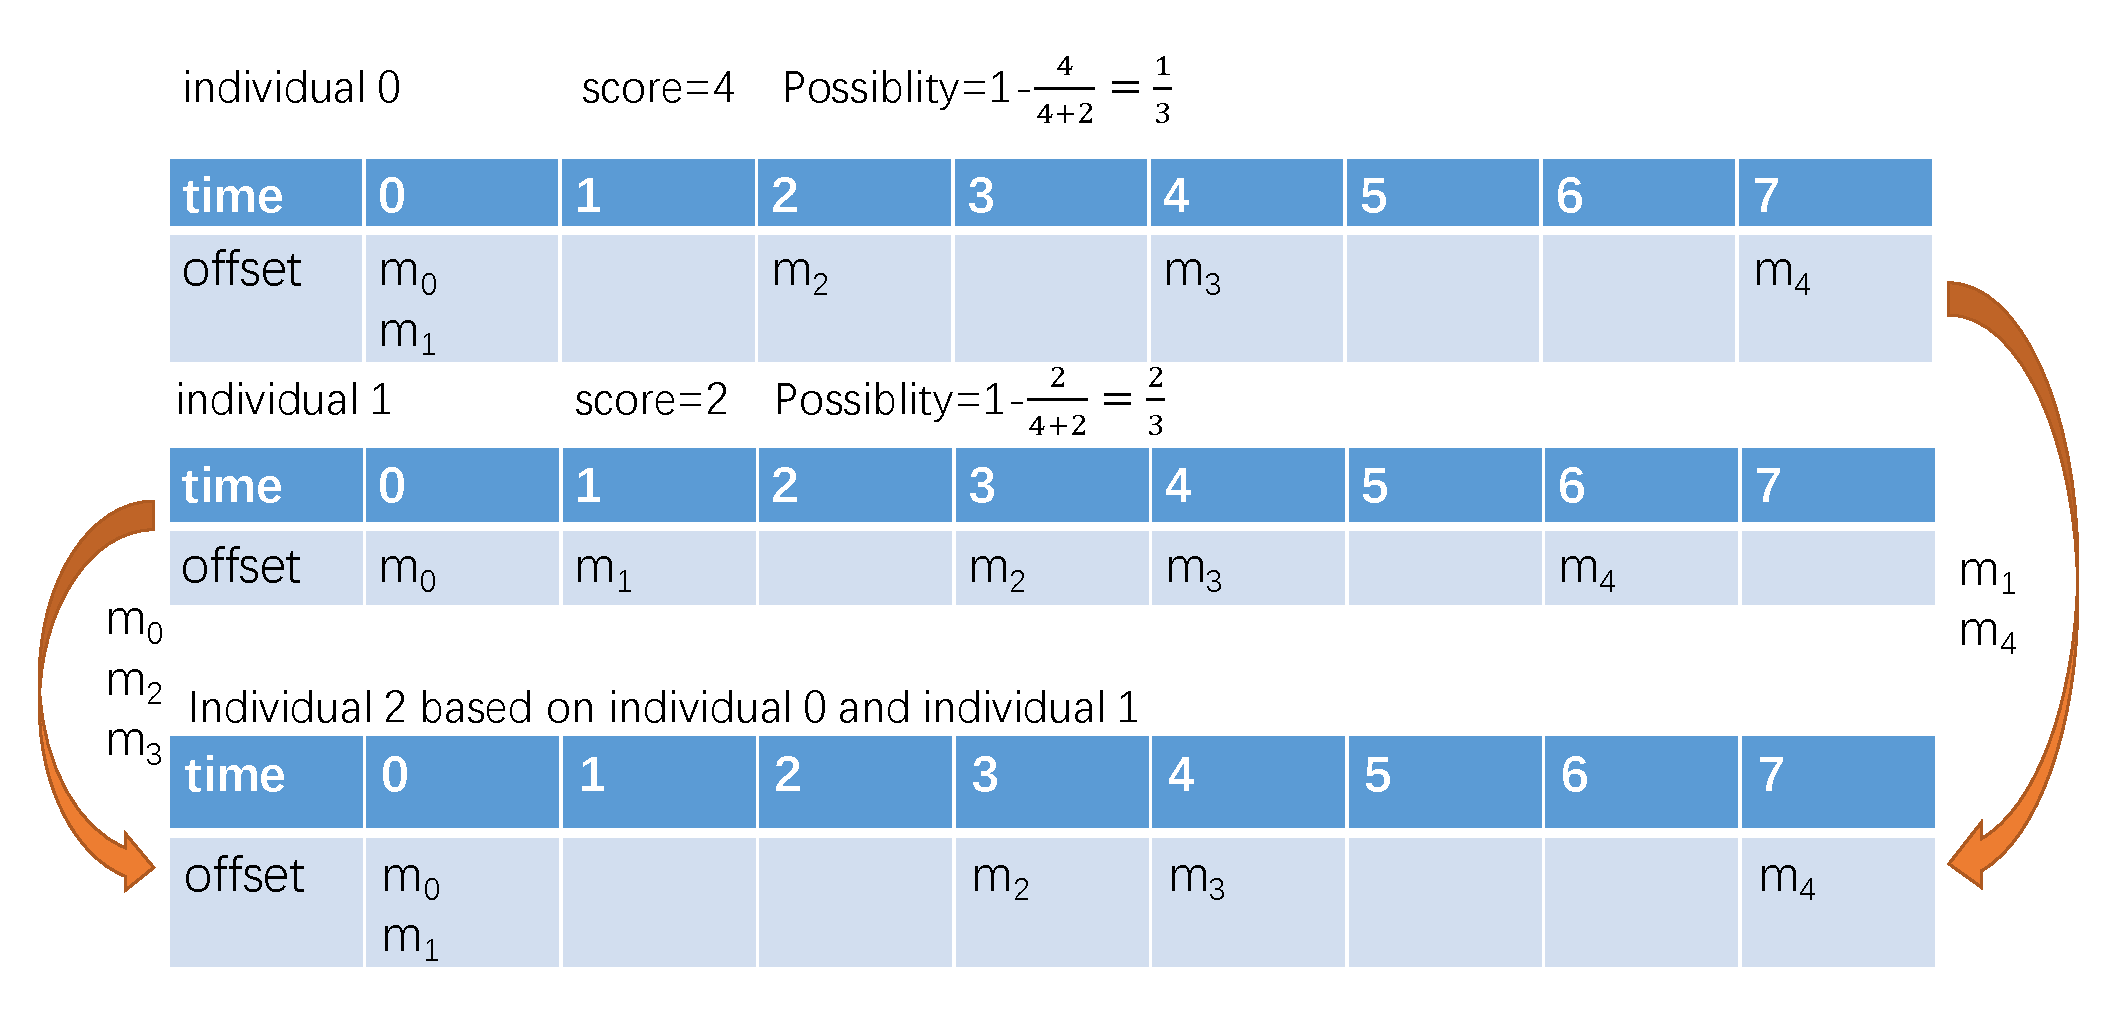
\includegraphics[width=3in]{picture/crossover.pdf}
%	\caption{An example of crossover employed individuals in Fig~\ref{t:pop} as parents}
%	\label{f:crossover}
%\end{figure}
\begin{table}[!t]
	\renewcommand{\arraystretch}{1.3}
	\newcommand{\tabincell}[2]{\begin{tabular}{@{}#1@{}}#2\end{tabular}}
	%if using array.sty, it might be a good idea to tweak the value of
	% \extrarowheight as needed to properly center the text within the cells
	\caption{An example of crossover employed individuals in Fig~\ref{t:pop} as parents}
	\label{t:crossover}
	\centering
	% Some packages, such as MDW tools, offer better commands for making tables
	% than the plain LaTeX2e tabular which is used here.
	\begin{tabular}{|c||c||c||c||c||c||c||c||c|}
		\hline
		\textbf{Parents}& 
		\textbf{0} & 
		\textbf{1} & 
		\textbf{2} & 
		\textbf{3} &
		\textbf{4} & 
		\textbf{5} & 
		\textbf{6} & 
		\textbf{7} \\		
		\hline
		$indi0$	&$m_0,m_1$&	&$m_2$&	&$m_3$& & &$m_4$\\		
		\hline		
		$indi1$	&$m_0$&$m_1$&	&$m_2$&$m_3$& &$m_4$&	\\		
		\hline
		\hline
			\textbf{Child}& 
			\textbf{0} & 
			\textbf{1} & 
			\textbf{2} & 
			\textbf{3} &
			\textbf{4} & 
			\textbf{5} & 
			\textbf{6} & 
			\textbf{7} \\		
			\hline
			$indi2$	&$m_0,m_1$&	& &$m_2$&$m_3$& & &$m_4$\\			
		\hline
	\end{tabular}
\end{table}

The operation of mutation random select an offset $s_i.\phi$ of scheduling $s_i\in\calS$.
Then selecting a new location of its offset randomly.
TABLE~\ref{t:mutation} is an example of mutation.
It is noted that the probability of mutation for each individual in our implement is 50\%.
%\begin{figure}[!t]
%	\centering
%	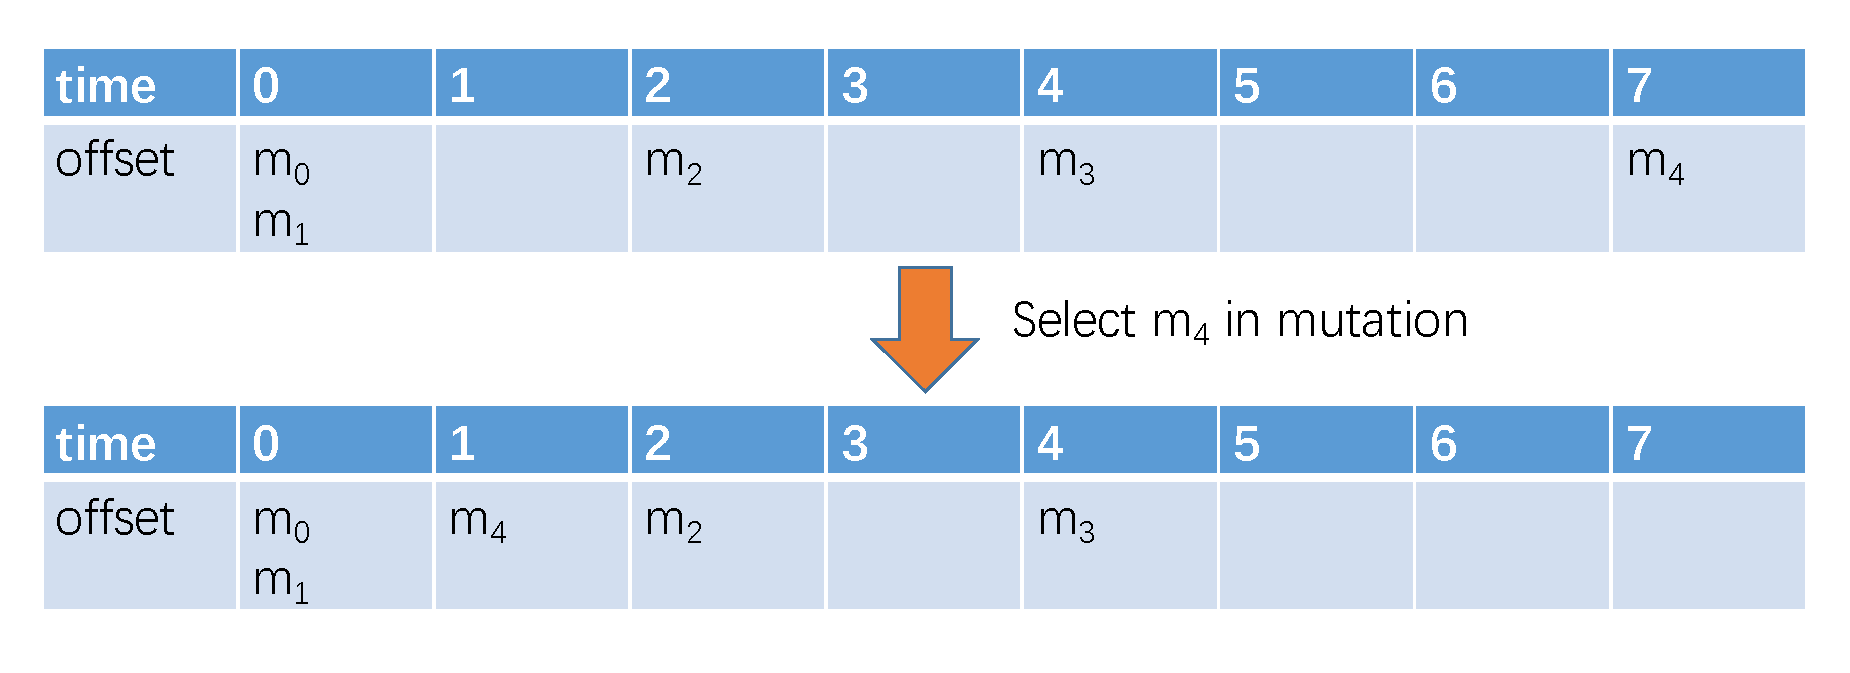
\includegraphics[width=3in]{picture/mutation.pdf}
%	\caption{An example of mutation}
%	\label{f:mutation}
%\end{figure}
\begin{table}[!t]
	\renewcommand{\arraystretch}{1.3}
	\newcommand{\tabincell}[2]{\begin{tabular}{@{}#1@{}}#2\end{tabular}}
	%if using array.sty, it might be a good idea to tweak the value of
	% \extrarowheight as needed to properly center the text within the cells
	\caption{An example of mutation}
	\label{t:mutation}
	\centering
	% Some packages, such as MDW tools, offer better commands for making tables
	% than the plain LaTeX2e tabular which is used here.
	\begin{tabular}{|c||c||c||c||c||c||c||c||c|}
		\hline
		\textbf{Before}& 
		\textbf{0} & 
		\textbf{1} & 
		\textbf{2} & 
		\textbf{3} &
		\textbf{4} & 
		\textbf{5} & 
		\textbf{6} & 
		\textbf{7} \\		
		\hline
		$indi0$	&$m_0,m_1$&	&$m_2$&	&$m_3$& & &$m_4$\\		
		\hline
		\hline
		\textbf{After}& 
		\textbf{0} & 
		\textbf{1} & 
		\textbf{2} & 
		\textbf{3} &
		\textbf{4} & 
		\textbf{5} & 
		\textbf{6} & 
		\textbf{7} \\		
		\hline
		$indi3$	&$m_0,m_1$&$m_4$&$m_2$&	&$m_3$& & &\\			
		\hline
	\end{tabular}
\end{table}


\subsection{Local search strategy \label{s:loc}}

Before the local search for each individual,
 the scheduling $s_i\in\calS$ with the maximum value of $times(s_i)$ is selected as local search element.
If there are two or more individuals with the maximum conflict times,
 the element to be searched is select stochastically among them.
Then the offset $s_i.\phi$ of selected $s_i$ is reallocated in its possible offset $s_i.\Phi$ .
Each reallocated individual is a candidate to update the previous individual.
After marking all of the candidate, the individual with minimum score replaces the previous individual.

TABLE~\ref{t:local} shows an example of local search for $indi0$ in Fig~\ref{t:pop}.
According to the $T(\calS)$ of individual 0 in TABLE~\ref{t:fitness},
 we random select $s_0$ as the element. 
Since the possible offset $s_i.\Phi$ of $s_0.\phi$ is 0 and 1 shown in TABLE~\ref{t:comm_info},
  we locate the the scheduling $s_0$ for message $m_0$ on its possible offset, gene 0 and gene 1 respectively.
After marking two of individual with different offset $s_0.\phi$,
 we select the individual which score is 2 as the updated $indi0$ because this individual own minimum score among the candidates which just reallocate the offset of $s_0$.
%\begin{figure}[!t]
%	\centering
%	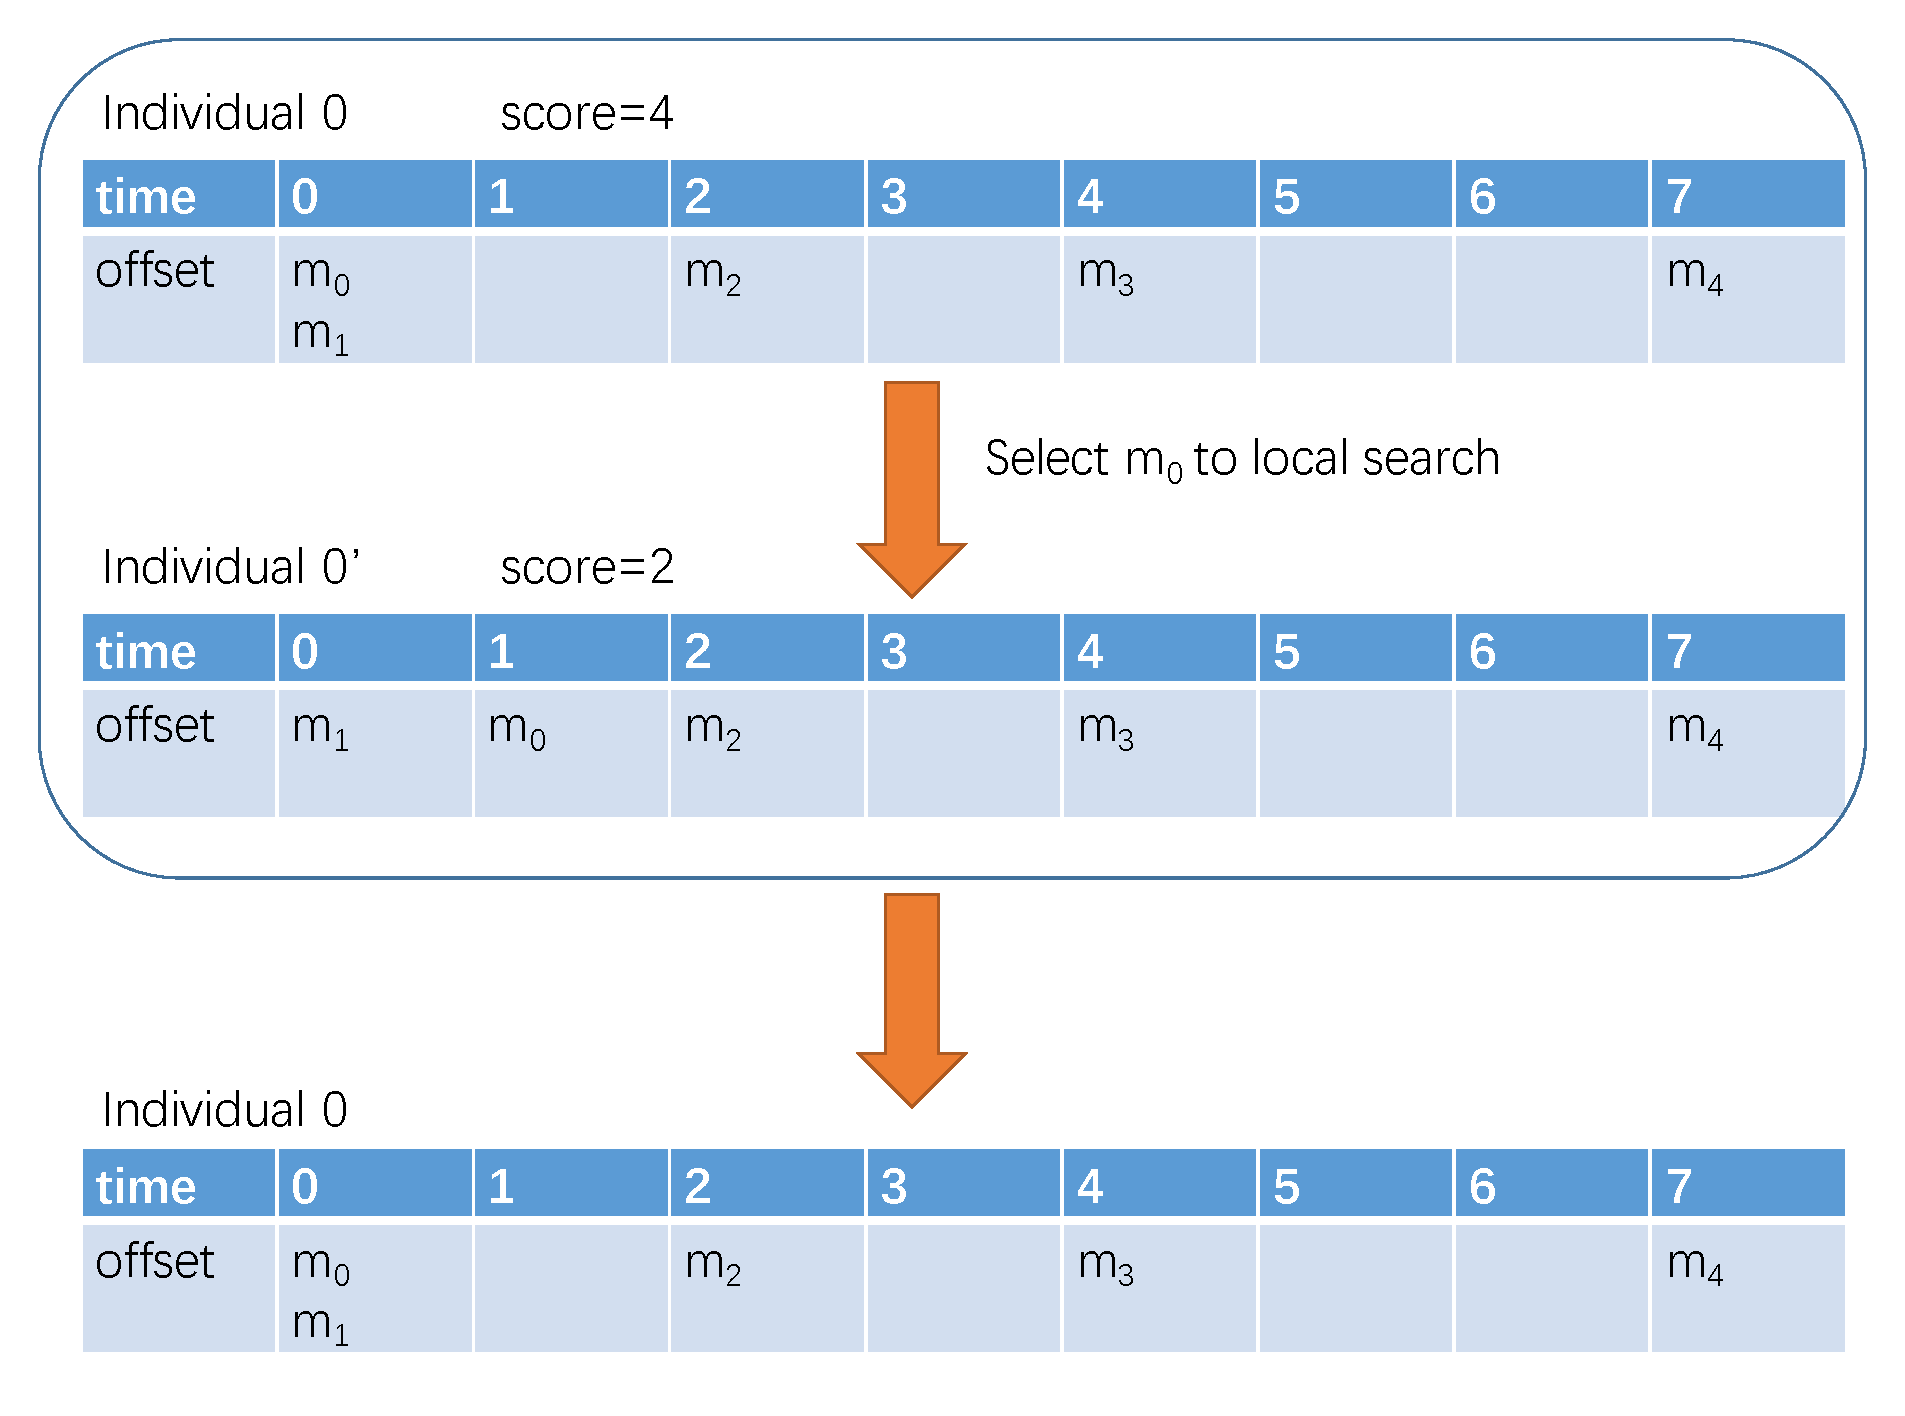
\includegraphics[width=3in]{picture/local.pdf}
%	\caption{An example of local search}
%	\label{f:local}
%\end{figure}
\begin{table}[!t]
	\renewcommand{\arraystretch}{1.3}
	\newcommand{\tabincell}[2]{\begin{tabular}{@{}#1@{}}#2\end{tabular}}
	%if using array.sty, it might be a good idea to tweak the value of
	% \extrarowheight as needed to properly center the text within the cells
	\caption{An example of local search of $m_0$ as element}
	\label{t:local}
	\centering
	% Some packages, such as MDW tools, offer better commands for making tables
	% than the plain LaTeX2e tabular which is used here.
	\begin{tabular}{|c||c||c||c||c||c||c||c||c|}
		\hline
		\textbf{Before}& 
		\textbf{0} & 
		\textbf{1} & 
		\textbf{2} & 
		\textbf{3} &
		\textbf{4} & 
		\textbf{5} & 
		\textbf{6} & 
		\textbf{7} \\		
		\hline
		$indi0$	&$m_0,m_1$&	&$m_2$&	&$m_3$& & &$m_4$\\		
		\hline
		\hline
		\textbf{Score}& 
		\textbf{0} & 
		\textbf{1} & 
		\textbf{2} & 
		\textbf{3} &
		\textbf{4} & 
		\textbf{5} & 
		\textbf{6} & 
		\textbf{7} \\		
		\hline
		$4$	&$m_0,m_1$&	&$m_2$&	&$m_3$& & &$m_4$\\
		\hline
		$2$	&$m_1$&$m_0$&$m_2$&	&$m_3$& & &$m_4$\\		
		\hline
		\hline		
		\textbf{After}& 
		\textbf{0} & 
		\textbf{1} & 
		\textbf{2} & 
		\textbf{3} &
		\textbf{4} & 
		\textbf{5} & 
		\textbf{6} & 
		\textbf{7} \\		
		\hline
		$indi0$&$m_1$&$m_0$&$m_2$&	&$m_3$& & &$m_4$\\		
		\hline
	\end{tabular}
\end{table}

In our implement,
 we naively traverse all the possible offset.
However for improving efficiency,
 many other algorithm in local search can be applied,
  i.e. tabu search, simulated annealing.
And different local search strategy may increase the performance of the memetic algorithm.

\section{EVALUATION\label{s:evalu}}

\subsection{Experiments Configuration}
%The mapping between a message and a communication node $\{ <\tau_{i} , v_{j}>\mid \tau_{i}\in\Gamma,v_{j}\in\mathcal{V} \}$ is given. Each message $\tau_{i}\in\Gamma$ is allocated to a specific process element(communication node) $v_{i}\in\mathcal{V}$, thus the source node $v_{a}$ and sink node $v_{b}$ in $(v_{a},v_{b})\in \mathcal{L}$ are determined.

%The routing strategy of each message is given. Therefore the link $(v_{a},v_{b})$ and the set of switches for forwarding the message is deterministic.To transmit a message $ \tau_{i}\in\Gamma $, the forwarding path is split in terms of hops by specific routing, i.e. $(v_{a},v_{b})=\{(v_{a},v_{s}),(v_{s},v_{n}),\dots,(v_{p},v_{q}),(v_{q},v_{b})\}$. 

%The switching technique is store-and-forward.

%The latency of forwarding in switch as well as the propagation latency on links is constant.

%In our experiment, for simplicity, the relative deadline is equal to the period for each message. The 2-ary mesh network is used and we randomly generate the mapping on the network. The X-Y routing is adopted as the routing strategy. And the relative deadline for each message equal its period. However the algorithm we introduced can be extended to resolve the scheduling problem with the general topology and arbitrary deterministic routing.


The network architecture we employed is 2D mesh network which scale is $3\times 3$, $5\times 5$ and $7\times 7$,
 with 9, 25 and 49 switching nodes respectively.
The program of our algorithm is implement in JAVA and is running on a Windows with 4GHz CPU and 12GB memory.
We compare the memetic algorithm with general genetic algorithm without local search. 

The number of scheduling of messages in our evaluation is from 5 to 50.
Each scheduling of message owns its period and delay which is random generated.
We test 15 cases in each scale of architecture with different number of messages.
The size of population we configure is 100.
Therefore there is 100 initial individual.
And the maximum iterate times we set is 100.
The memetic algorithm will finish if there is a feasible scheduling,
 otherwise the algorithm will execute until the iterate 100 times.
The case which executes exceeds an hour will be regarded as \emph{overtime}.

\subsection{Failed Scheduling Rate}
We define the failed scheduling of messages as the minimum number of messages.
The messages which failed to scheduling block the scheduling of other messages.
If the set of failed communication is removed from the given communication set on the TTNoC,
 the remaining messages will be scheduled.

Fig~\ref{f:fail} shows the rate of failed messages in the set of communication for variable type of test case. 
It should be noted that the rate is the average rate of the 15 test cases.
As can be seen,
 though the general algorithm spends quite a few time,
  the rate of failed scheduled messages is much more than the memetic algorithm, especially when the scale of communication set is relatively large.
E.g. for the case of 50 messages in $3\times 3$ TTNoC,
 the failed communication percentage is 17.3\% for genetic algorithm while 8\% for memetic algorithm.
  Therefore the local search in the memetic algorithm is the key step in memetic algorithm to significantly improve the performance of genetic algorithm.

And it is clear that the failed scheduling rate decreases when the scale of TTNoC architecture is larger. 
The reason of this result is that the link resource increases with the growth of architecture,
 resulting of decreasing the possibility of contention among the messages transmission on the TTNoC.
It also presents that the failed communication rate increases when the number of messages on the TTNoC increasing.
It is because that the limited link resources have to transmit more messages when there is more communication on the TTNoC.

To compare the performance of the general genetic algorithm and memetic algorithm,
 we define $MA/GA$ to represent the failed scheduling decreasing comparing MA and GA.
TABLE~\ref{t:performance} depicts the failed scheduling decrease of MA compared with GA.
As we can see, The rate of failed scheduling by MA is about 30\% of the rate by GA.

\begin{figure}[!t]
	\centering
	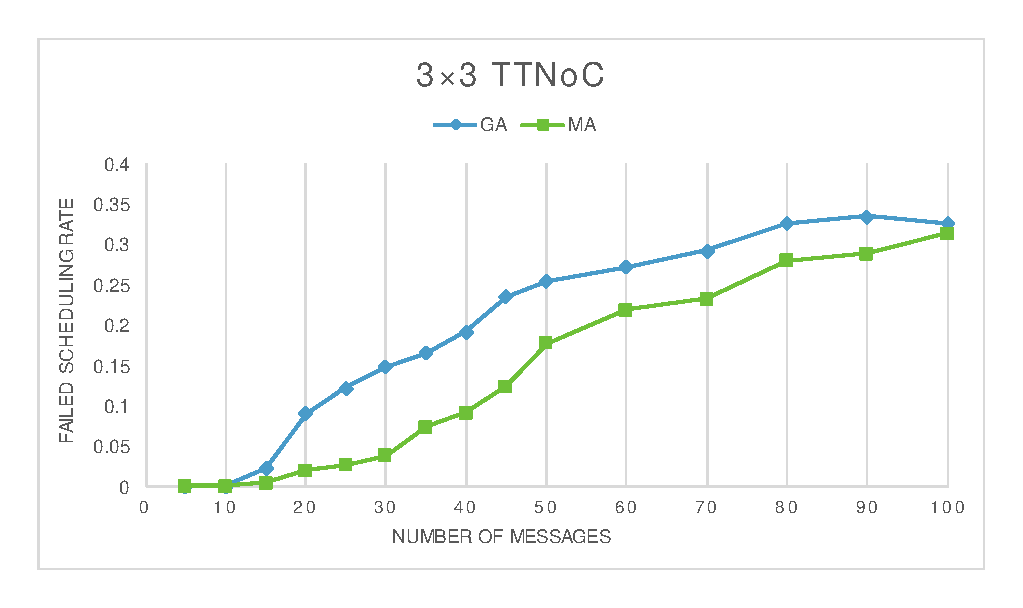
\includegraphics[width=3in]{picture/33TTNOC}
		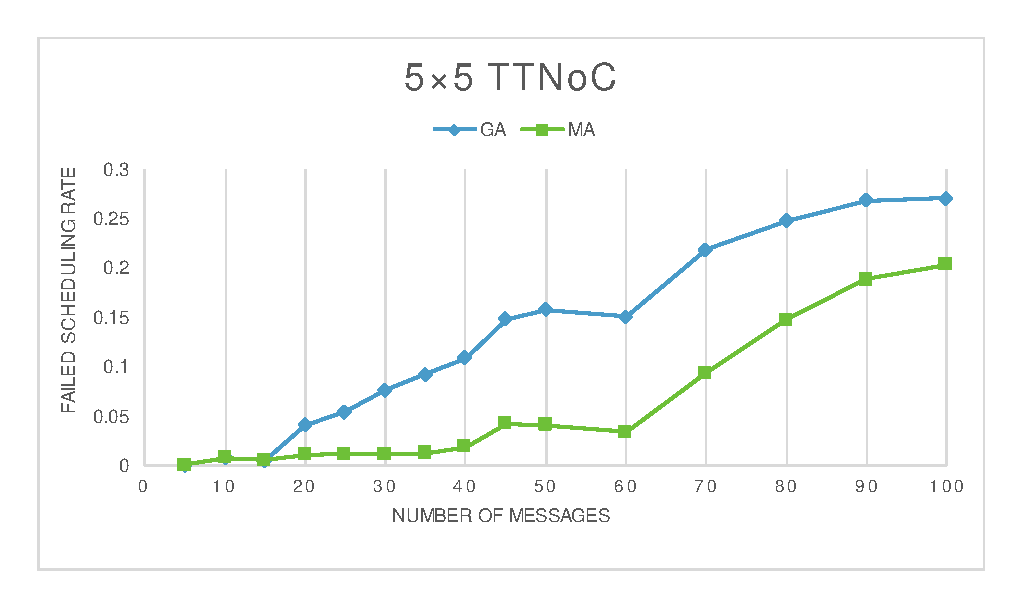
\includegraphics[width=3in]{picture/55TTNOC}
			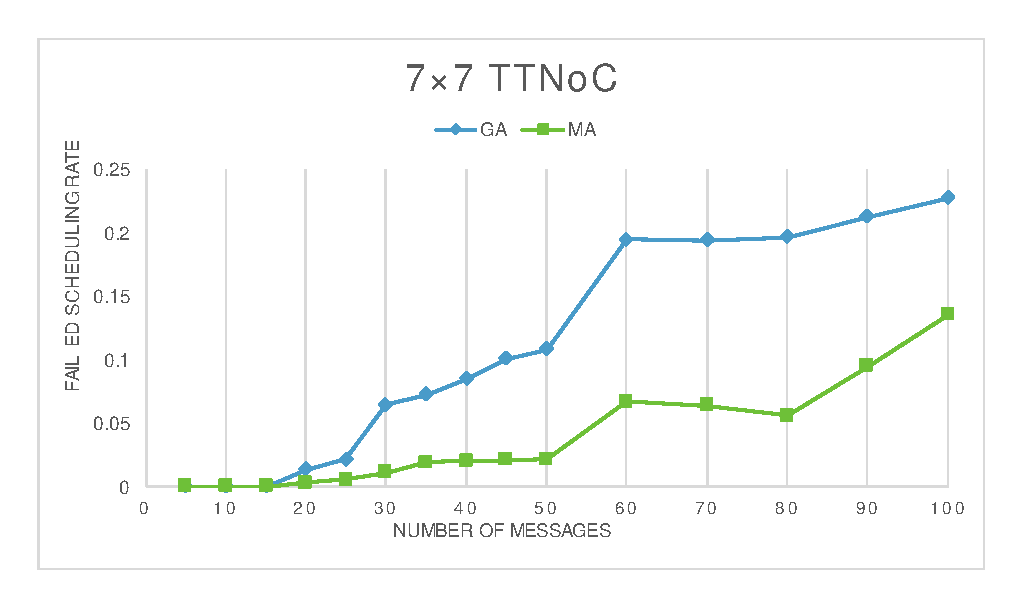
\includegraphics[width=3in]{picture/77TTNOC}
	\caption{The rate of failed scheduling}
	\label{f:fail}
\end{figure}

\subsection{Feasible Cases}
\begin{table}[!t]
	\renewcommand{\arraystretch}{1.3}
	%if using array.sty, it might be a good idea to tweak the value of
	% \extrarowheight as needed to properly center the text within the cells
	\caption{The average rate of failed scheduling in different architecture }
	\label{t:performance}
	\centering
	% Some packages, such as MDW tools, offer better commands for making TABLEs
	% than the plain LaTeX2e tabular which is used here.
	\begin{tabular}{|c||c||c||c|}
		\hline
		\textbf{Architecture} & \textbf{MA} &\textbf{GA} & \textbf{MA/GA}\\
		\hline 
		$3\times 3$ TTNoC&0.0557& 0.1232&	0.4521		
		\\
		\hline
		$5\times 5$ TTNoC& 0.0154	& 0.0685&0.2248\\
		\hline
		$7\times 7$ TTNoC& 0.010& 	0.0465&	0.2165\\
		\hline		
		\hline
		\textbf{Average }& 	0.0271 &0.0794&0.2978\\
		\hline
	\end{tabular}	
\end{table}
We consider the number of feasible case in each experiment type.
The case is successful if all the communication are scheduled in feasible location without link contention,
 otherwise we consider the case is infeasible case.
Fig~\ref{f:feasible} presents the result of number of feasible cases after schedule synthesis.
For simple test cases with less than 15 communication,
 almost cases is feasible.
But for complexed test cases more than 30 messages, it is hard for the algorithms to find a feasible scheduling.
\begin{figure}[!t]
	\centering
	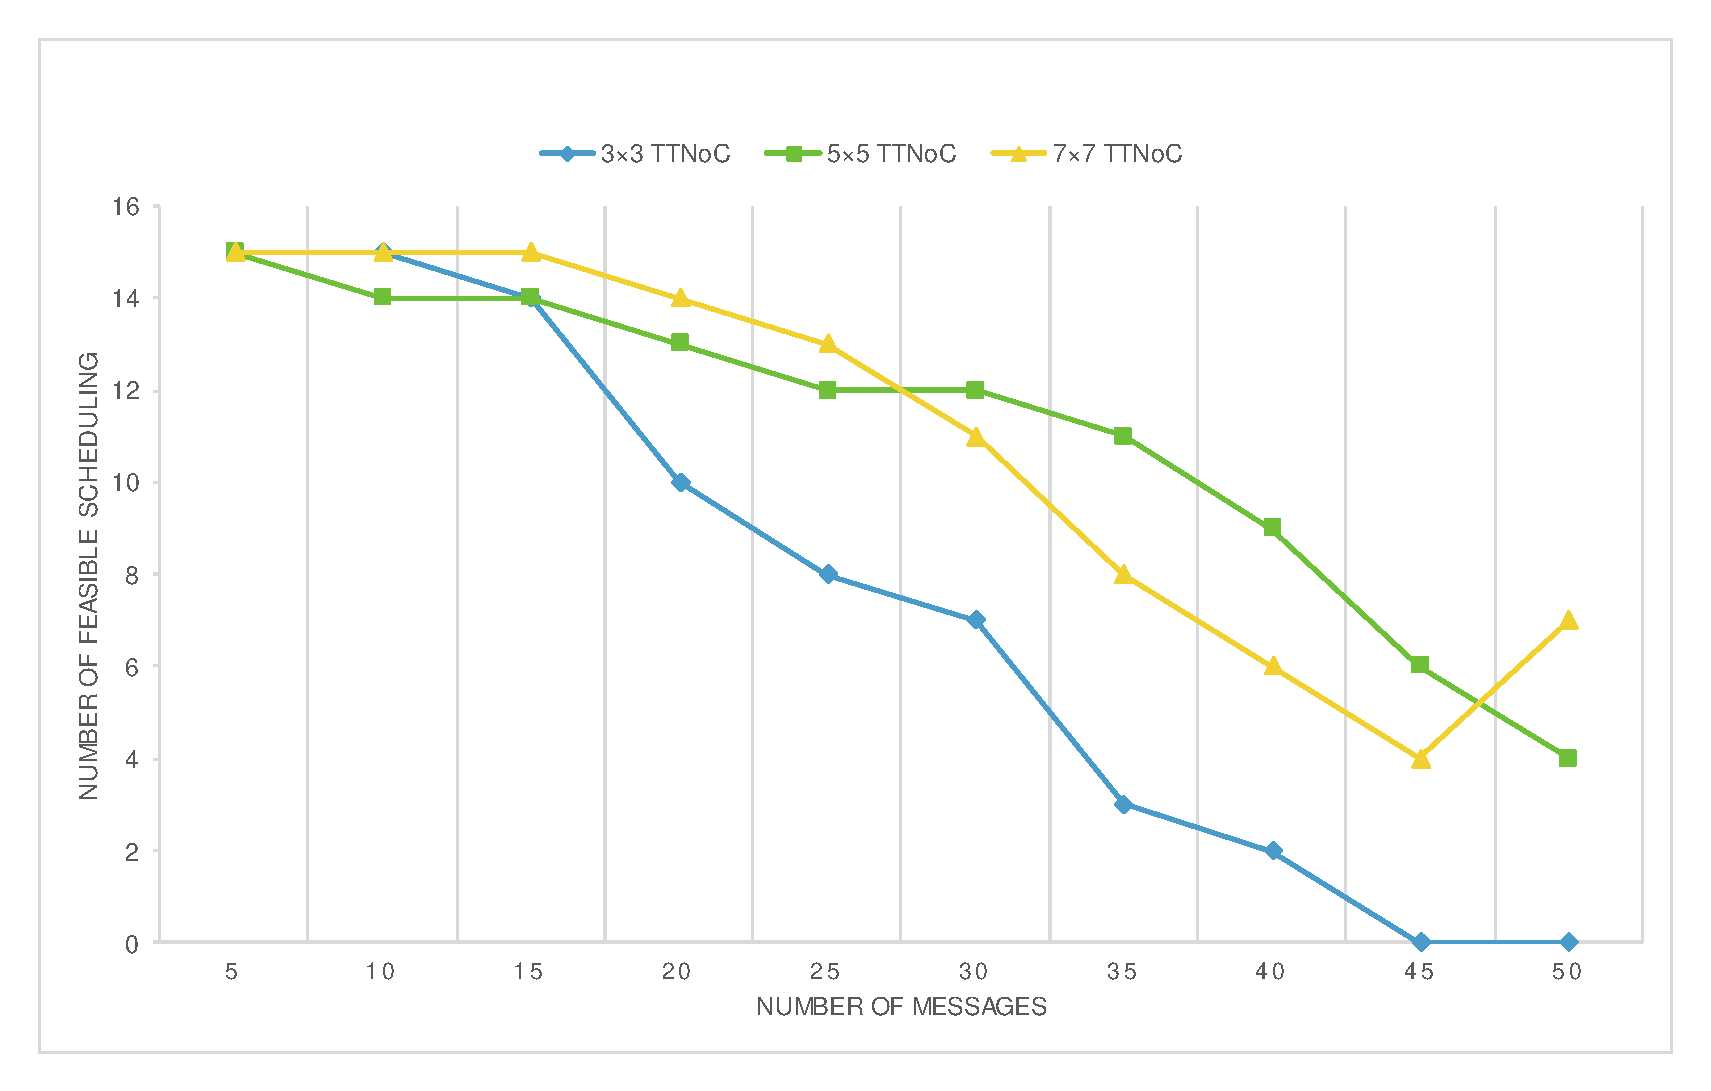
\includegraphics[width=3in]{picture/feasible_case}
	\caption{The number of feasible cases in different test cases}
	\label{f:feasible}
\end{figure}

\subsection{Discussions}

Synthesizing a feasible scheduling depends on the number of communication and the scale of TTNoC.
It is hard for memetic algorithm to synthesize a feasible scheduling when the set of communication is large and/or the TTNoC architecture is small.
However,
 except two reason above,
  the mapping between a message and a communication node and routing strategy of communications also affect generating a feasible solution.
Therefore the designer can manually change the map allocation or the routing strategy to the failed scheduling,
 and even design a larger network architecture if needed.
After these change,
   the feasible scheduling can be generated by the memetic algorithm iteratively. 

\section{CONCLUSION\label{s:conclud}}

This paper introduces a memetic algorithm to resolve the message scheduling problem on the TTNoC.
We verify our memetic algorithm with on various random generated messages on different scales of TTNoC.
The experiment results shows that our memetic algorithm is efficient to synthesize a scheduling with high percentage of scheduled messages.

In our future work,
the mapping between messages and nodes and routing strategy may be integrated to the TTNoC scheduling.
And the different TTNoC architecture,
i.e. torus, hypercube,
and different local search strategy can be also considered in our experiment.




% conference papers do not normally have an appendix


% use section* for acknowledgment
%\section*{Acknowledgment}
%The authors would like to thank...





% trigger a \newpage just before the given reference
% number - used to balance the columns on the last page
% adjust value as needed - may need to be readjusted if
% the document is modified later
%\IEEEtriggeratref{8}
% The "triggered" command can be changed if desired:
%\IEEEtriggercmd{\enlargethispage{-5in}}

% references section

% can use a bibliography generated by BibTeX as a .bbl file
% BibTeX documentation can be easily obtained at:
% http://mirror.ctan.org/biblio/bibtex/contrib/doc/
% The IEEEtran BibTeX style support page is at:
% http://www.michaelshell.org/tex/ieeetran/bibtex/
%\bibliographystyle{IEEEtran}
% argument is your BibTeX string definitions and bibliography database(s)
%\bibliography{IEEEabrv,../bib/paper}
%
% <OR> manually copy in the resultant .bbl file
% set second argument of \begin to the number of references
% (used to reserve space for the reference number labels box)
%% \begin{thebibliography}{1}

%% \bibitem{IEEEhowto:kopka}
%% H.~Kopka and P.~W. Daly, \emph{A Guide to \LaTeX}, 3rd~ed.\hskip 1em plus
%%   0.5em minus 0.4em\relax Harlow, England: Addison-Wesley, 1999.

%% \end{thebibliography}

\bibliographystyle{IEEEtran}
\balance
\bibliography{main}


% that's all folks
\end{document}


